\documentclass[onecolumn, twoside, a4paper, 11pt]{memoir}

\usepackage[utf8]{inputenc}
\usepackage[T1]{fontenc}

% Fonts
\usepackage{newpxtext,newpxmath}
\renewcommand*\sfdefault{cmss}

% References
\usepackage{hyperref}

% Fancy command for auto-refing multiple references
\makeatletter
\newcommand\Autoref[1]{\@first@ref#1,@}
\def\@throw@dot#1.#2@{#1}% discard everything after the dot
\def\@set@refname#1{%    % set \@refname to autoefname+s using \getrefbykeydefault
    \edef\@tmp{\getrefbykeydefault{#1}{anchor}{}}%
    \def\@refname{\@nameuse{\expandafter\@throw@dot\@tmp.@autorefname}s}%
}
\def\@first@ref#1,#2{%
  \ifx#2@\autoref{#1}\let\@nextref\@gobble% only one ref, revert to normal \autoref
  \else%
    \@set@refname{#1}%  set \@refname to autoref name
    \@refname~\ref{#1}% add autoefname and first reference
    \let\@nextref\@next@ref% push processing to \@next@ref
  \fi%
  \@nextref#2%
}
\def\@next@ref#1,#2{%
   \ifx#2@ and~\ref{#1}\let\@nextref\@gobble% at end: print and+\ref and stop
   \else, \ref{#1}% print  ,+\ref and continue
   \fi%
   \@nextref#2%
}
\makeatother

% URL styles
\usepackage{url}
\urlstyle{sf}

% Units
\usepackage[detect-weight=true, binary-units=true]{siunitx}
\DeclareSIUnit\flop{Flops}

% Math
\usepackage{amsmath}
\usepackage{amssymb}
\usepackage{bm}

\newtheorem{ex}{Exercise}[chapter]

% Graphics
\usepackage{graphicx}
\graphicspath{{figs/}}

% Tikz
\usepackage{tikz}
\usetikzlibrary{positioning,shapes,arrows,calc,intersections}
\usepackage{pgfplots}
\usepgfplotslibrary{dateplot}
\pgfplotsset{compat=1.8}

% Colors
\definecolor{darkblue}{HTML}{00688B}
\definecolor{darkgreen}{HTML}{6E8B3D}
\definecolor{cadet}{HTML}{DAE1FF}
\definecolor{salmon}{HTML}{FFB08A}

% Listings
\usepackage{textcomp}
\usepackage{listings}
\lstset{
  keywordstyle=\bfseries\color{orange},
  stringstyle=\color{darkblue!80},
  showstringspaces=false,
  basicstyle=\ttfamily,
  upquote=true,
}
\lstdefinestyle{fortran}{
  language=Fortran,
  morekeywords={for},
  deletekeywords={status},
}
\lstdefinestyle{c}{
  language=C,
  morekeywords={include},
}
\lstdefinestyle{shell}{
  language=bash,
}

% Double hlines
\usepackage{hhline}

% Make footnotes work inside tables
\usepackage{footnote}
\makesavenoteenv{tabular}
\makesavenoteenv{table}

% Numbering
\makeatletter
\AtBeginDocument{%
  \let\c@lstlisting\c@figure
  \let\c@table\c@figure
}
\makeatother

\begin{document}

\begin{titlingpage}
  \centering
  {\Huge \bfseries \scshape
    Introduction to \\[0.2\baselineskip] Supercomputing} \\[2\baselineskip]
  {\Large TMA4280} \\[0.7\textheight]
  \copyright \\
  Einar R{\o}nquist \\
  Arne Morten Kvarving \\
  Eivind Fonn
\end{titlingpage}

\chapter{Introduction}

\section{Supercomputing}

What do we mean by supercomputing? In general, we mean using computers to solve
problems which are very computationally intensive, i.e. problems which require
large computing resources in terms of memory or floating-point operations, or
both. Examples of problems requiring supercomputing are weather forecasting
(\url{http://met.no} uses the supercomputing facility here at NTNU), oil
exploration (reservoir simulation), seismic analysis (an inverse problem),
computational chemistry, computational physics, computational mechanics (e.g.
structural mechanics, fluid mechanics) and material science.

Due to the resource demanding aspects of supercomputing, it is important to make
the whole solution process as efficient as possible. Examples of important
issues to study are:
\begin{itemize}
\item numerical and computational algorithms which are fast, robust and accurate
\item software development
\item treatment of large data sets
\item visualization
\item validation of the simulation results
\end{itemize}
Supercomputing typically implies the use of parallel processing. This means that
the underlying algorithms used need to be designed and tuned for such a
computing environment. The software development typically becomes more involved
compared to a single-process implementation even though the trend is to abstract
the machine specific details as much as possible.

Because of the compute-intensive (memory, floating-point, I/O) nature of these
problems, they often require special high-end computing platforms. In Norway,
there is at least one such system at each major university. The large oil
companies in Norway also have such computing platforms. Each system is still
quite expensive to purchase, to operate and to maintain. In addition, special
intrastructure often needs to be built around such systems: special rooms
(security), power supply, cooling systems etc. Due to the overall investment,
both in terms hardware and in terms of human resources, it is important to use
these systems as efficiently as possible---each system typically lasts only a
few years.

Even if the current systems are powerful, it is important to make progress in
terms of making such systems easier to build and to use, and to develop more
efficient computational algorithms. This will enable larger and more realistic
problems to be simulated, which translates into progress in science and
engineering (which are the ``classical'' applications for supercomputing), but
also in other emerging areas such as the medical field.

In the following, let us briefly mention some of the issues involved when
working with a specific application. Assume that we have a program for
simulating the blood flow through part of a vein. Let $T_1$ be the solution time
on a single processor (even though, in reality, such a simulation would probably
not fit on a single-processor machine).

Assume now that we port this simulation to a multi-processor system with $P$
processors. Ideally, we would like the solution time to be reduced by a factor
of $P$. Another way of saying this is that we would like to achieve a speedup
\begin{align}
  S_p=T_1/T_p = P,
\end{align}
where $T_p$ is the solution time on $P$ processors. Typically, the speedup $S_p
< P$. As we increase the number of processors to solve our particular (fixed)
problem, we will first see a good speedup, followed by a degradation as we add
more and more processors. The main explanation for this is easy to understand.
In order to achieve a perfect speedup, we cannot have any overhead when moving
from a single processor system to a multi-processor system. In reality, we have
communication between the processors. As the number of processors is increased,
the work per processor goes down, while the overall communication overhead goes
up. A critical issue is therefore to minimize the communication overhead so that
we can take advantage of larger systems for a fixed problem.

We should here remark that one of the major advantages of having access to a
supercomputing facility is the possibility to solve much larger problems than
what is possible on a smaller system. Hence, as we increase the number of
processors, we may also increase the problem size so that the work per processor
remains fixed. We will consider some of these issues in this course.

Let us now discuss the single-processor performance a bit more. Assume for the
moment that we have two different versions (executables), $A$ and $B$, of a
particular application. We also assume that the underlying numerical algorithms
are identical. The simulation times for the two versions are denoted as $T_1^A$
and $T_1^B$, respectively. We observe that
\begin{align}
  T_1^A = 3 T_1^B.
\end{align}
Why are the two simulation times so different since the numerical algorithms are
the same?

\begin{figure}
  \centering
  \begin{tikzpicture}
    \matrix[
    column sep=4mm,
    every node/.style={
      shape=rectangle,
      rounded corners=1mm,
      draw=darkblue,
      fill=cadet,
      minimum height=1cm,
      text width=2.5cm,
      text centered,
      text height=1.5ex,
      text depth=.25ex,
    }]{
      \node (alg) {Algorithm}; &
      \node (prog) {Programming}; &
      \node (comp) {Compiler}; &
      \node (exe) {Executable}; \\
    };
    \begin{scope}[->, darkblue, thick]
      \draw (alg) -- (prog);
      \draw (prog) -- (comp);
      \draw (comp) -- (exe);
    \end{scope}
  \end{tikzpicture}
  \caption{Ingredients in a simulation.}
  \label{fig:single}
\end{figure}

We only mention a few aspects which may have caused this; see Figure \ref{fig:single}:
\begin{itemize}
\item different choice of data structure / memory layout during the programming;
\item different use of optimized numerical libraries;
\item different choices of compiler optimization.
\end{itemize}
We will look at some of these issues in this course.
Note that it is typically harder to achieve a good speedup for version B compared to
version A, even though $T_1^B  < T_1^A$ (can you suggest a reason why?)

Are there other ways to change the solution time for our particular simulation?
Yes; we mention two distinct ways:
\begin{itemize}
\item change the computer;
\item change the computational or numerical algorithms.
\end{itemize}
Progress in the available hardware has been impressive over the past decades.
However, it is important to realize that progress in computational algorithms
has been equally impressive. Note that developing a new algorithm which requires
only half the number of floating point operations is equally important as buying
a new computer with twice the performance in terms of floating point operations
per second (Flops).

We will discuss a few selected numerical algorithms in this course, e.g.
numerical solution of partial differential equations (primarily finite
difference methods), iterative and direct methods for solving linear systems of
equations, basic linear algebra routines, and a little bit about statistical
methods (Monte Carlo methods).

\section{Floating point representation}

This section gives a brief introduction to the IEEE standard (IEEE-754) for
floating point representation. A basic understanding of the standard is
appropriate given the importance of floating point operations in this course.

All real numbers are represented with a finite number of bits. The
representation is depicted in Figure \ref{fig:fp}. The sign bit is certainly
easy to understand. A value $S=0$ means that the number is positive, while a
value $S=1$ means that the number is negative.

\begin{figure}
  \centering
  \begin{tikzpicture}[scale=0.5]
    \draw (0,0) rectangle (1,1);
    \draw (1,0) rectangle (7,1);
    \draw (7,0) rectangle (20,1);
    \node at (0.5, 0.5) {$S$};
    \node at (4, 0.5) {$E$};
    \node at (13.5, 0.5) {$F$};
  \end{tikzpicture}
  \caption{
    Each floating point has a binary representation with three fields: $S$
    denotes the sign of the number, $E$ is an exponent, and $F$ is the fraction
    part of the mantissa.
  }
  \label{fig:fp}
\end{figure}

The actual decimal value $V$ of the floating point is
\begin{align}
  V = (-1)^S \cdot 2^{E-B}\cdot M
\end{align}
where $M$ is the mantissa and $B$ is denoted as the \emph{bias} which will be
explained below. The exponent E is always adjusted such that the mantissa can be
expressed as
\begin{align}
  M = \underbrace{1}_{\times2^0} .
  \overbrace{\underbrace{b_1}_{\times2^{-1}}
  \underbrace{b_2}_{\times2^{-2}}\ldots}^{F}
\end{align}
where $F$ denotes the fraction of the mantissa in binary representation (i.e.
the binary digits $b_1b_2\ldots$). Since this representation is always assumed,
the binary number $1$ in the front is not explicitly represented. Note that,
\begin{align}
  1 \leq M < 2,
\end{align}
since the fraction $F$ is always less then one.

There are many more details regarding floating point representation. For
example, the implicitly assumed binary number 1 in the mantissa is only true for
what is referred to as {\em normalized} numbers.

\begin{table}
  \centering
  \caption{Number of bits for common floating point standards.}
  \bgroup\def\arraystretch{1.2}
  \begin{tabular}{ccccc} \hline
    Precision & $S$ & $E$ & $F$ & Total \\ \hhline{=====}
    Single & $1$ & $8$ & $23$ & 32
    \\ \hline
    Double & $1$ & $11$ & $52$ & 64
    \\ \hline
  \end{tabular}
  \egroup
\end{table}

A few words about the exponent $E$. In single precision, $E$ is represented
using 8 bits, giving 256 possibilities, of which 254 are used to represent
normalized numbers. The values $E=0$ and $E=255$ are primarily reserved for zero
and infinities. The actual exponent used to find the corresponding decimal value
of a normalized number is $E-B$; see equation (1). For single precision,
$B=127$ and for double precision, $B=1023$.

We can now compute the maximum and minimum numbers that we can represent in
single precision (i.e. using 32 bits):
\begin{alignat}{2}
  \label{maxnumber}
  V_{\text{max}} &= 1 \cdot 2^{254-127} \cdot 2 &&\approx 3.40 \cdot 10^{38} \\
  \label{minnumber}
  V_{\text{min}} &= 1\cdot 2^{1-127} \cdot 1 &&\approx 1.17 \cdot 10^{-38}
\end{alignat}
As we can see, this is a significant range.

Having considered the range, let us now consider the accuracy of a given
floating point number. Again, consider the single precision case. The fraction
of the mantissa is represented using 23 bits, meaning that the smallest {\em
fraction} that can be represented is
\begin{align*}
  2^{-23} \approx 1.19 \cdot 10^{-7}.
\end{align*}
This implies that {\em any} floating point number using single precision
(covering the whole range discussed above) has about 7 digits of accuracy.

\begin{ex}
  Consider the maximum and minimum numbers defived in
  \eqref{maxnumber}-\eqref{minnumber}. How many digits should we include in each
  of these numbers when written out?
\end{ex}

\begin{ex}
  Find the binary floating point representation of the decimal number $4.25$ in
  single precision.
\end{ex}

\begin{ex}
  How many decimal digits of accuracy does a double precision floating point
  number have?
\end{ex}

\section{Integer representation}

An integer is typically represented using 32 bits. One bit is used to represent
the sign. Hence, the possible integers will be in the range $\pm 2^{31} \approx
\pm 2\cdot 10^9$.

If an algorithm includes a loop which needs to be done $n$ times (e.g., a Monte
Carlo simulation), $n$ needs to be less than approximately $10^9$. This may seem
sufficient, however, there could be situations when this limitation could become
an issue.

\begin{ex}
  Propose one or several ways around this limitation.
\end{ex}

\section{Floating point performance}

The basic operations of adding, multiplying, subtracting and dividing two
floating point numbers are counted as floating point operations.

Floating point performance is usually measured in number of floating point
operations per second, commonly abbreviated as Flops; for a brief discussion
see \url{http://en.wikipedia.org/wiki/FLOPS}.

Since current computer systems typically perform many of these operations per
seconds, abbreviations like MFlops (megaflops), GFlops (gigaflops), TFlops
(teraflops), and PFlops (petaflops) are common to use.

When we speak about the speed of a computer, we will typically mean the floating
point performance.

\begin{ex}
  Let $c$ be a scalar (a floating point number), let $\bm x$, $\bm y$, and $\bm
  z$ be vectors, each comprising $n$ floating point numbers, and let $\bm A$ be
  an $n\times n$ matrix. How many floating point operations does it take to
  perform the following basic linear algebra operations?
  \begin{align*}
  \bm z = \bm x + c \bm y, \qquad \bm y = \bm A \bm x
  \end{align*}
\end{ex}

\section{Storage requirements}

It is quite common today to do all the necessary computations using double
precision. This means that 64 bits are used to represent each floating point
number, which is equivalent to 8 bytes (8 bits per byte).

Let us now consider how many floating point numbers we can store in the memory
associated with a typical processor. Assume that we have available
$\SI{4}{\giga\byte}$ ($4\cdot 10^9$ bytes) of main memory (or RAM: \emph{Random
Access Memory}); this is a quite typical size nowadays. This amount of memory is
sufficient to represent a total of 512 millon floating point numbers in double
precision.

In practice, we could never use the entire memory for such a purpose. We also
need space for our simulation program (instructions etc.). However, it gives an
indication of the order of magnitude that we can handle.

If we are solving differential equations or some other problem, we also need to
use memory to store matrices, temporary variables, etc. The available memory to
store the actual solution depends on the numerical algorithm, however even a
fairly scalable algorithm would typically only be able to handle a few million
unknowns. Many algorithms would allow far fewer unknowns.

Problems in science and engineering can easily require many million unknowns,
perhaps even billions of unknowns. In order to solve such problems, we obviously
need both more memory and increased computing power. This is achieved using
parallel processing where multiple processors and memory modules are connected
into a single computational platform.

\begin{ex}
  Let $\bm A$ be an $n\times n$ matrix, and $\bm x$ and $\bm b$ be two vectors
  of length $n$. Assume that we want to solve the linear system of equations
  \begin{align*}
    \bm A \bm x = \bm b
  \end{align*}
  using Gaussian elimination. Assume further that the matrix $\bm A$ is dense,
  meaning that we need to store all the $n^2$ entries in the matrix.

  What is (approximately) the largest equation system we can solve (i.e., the
  largest number of $n$ we can use) and still be able to fit the whole problem
  in the main memory, which we assume is $\SI{1}{\giga\byte}$?
\end{ex}

\section{Past, current and future supercomputers}

\autoref{fig:perform-dev} depicts the past and future performance development
of the 500 fastest supercomputers in the world. More information about the top
500 systems can be found on \url{http://top500.org}.

In 1986 a supercomputing center was established at NTH.
\autoref{tab:history-ntnu} gives a summary of the supercomputers at NTH/NTNU
since then.

\begin{figure}
  \centering
  \begin{tikzpicture}
  \begin{axis}[
    date coordinates in=x,
    ymode=log,
    xticklabel=\year,
    xmin=1993-05-01,
    xmax=2015-10-01,
    width=0.8\textwidth,
    height=0.6\textwidth,
    ytick={1, 1000, 1000000, 1000000000},
    yticklabels={$\SI{1}{\giga\flop}$, $\SI{1}{\tera\flop}$, $\SI{1}{\peta\flop}$, $\SI{1}{\exa\flop}$},
    grid=major,
    legend style={at={(1,0)}, anchor=south east},
    legend cell align=left,
    ]
    \addplot[mark=o, mark size=1.3, draw=darkgreen, thick]
    table[x=date, y=sum, col sep=comma]
    {\data/performance-development.csv};
    \addplot[mark=o, mark size=1.3, draw=red, thick]
    table[x=date, y=high, col sep=comma]
    {\data/performance-development.csv};
    \addplot[mark=o, mark size=1.3, draw=magenta, thick]
    table[x=date, y=low, col sep=comma]
    {\data/performance-development.csv};
    \legend{Sum, Highest, Lowest};
  \end{axis}
\end{tikzpicture}

  \caption{
    The performance development since 1993 for the top 500 supercomputers in the
    world. In particular, the figure indicates the performance development for
    the fastest system (number 1), the slowest system (number 500), and the sum
    of all the 500 fastest systems.
  }
  \label{fig:perform-dev}
\end{figure}

\begin{table}
  \caption{
    Supercomputers at NTH/NTNU. Note that some of this information is guesswork
    as not all machines were not available at when revising this document.
  }
  \centering
  \bgroup\def\arraystretch{1.2}
\begin{tabular}{llrlr}
  \hline
  Year & System & Processors & Type & $\SI{}{\giga\flop}$ \\
  \hhline{=====}
  1986--1992 & Cray X-MP & 2 & Vector & 0.5 \\
  1992--1996 & Cray Y-MP & 4 & Vector & 1.3\\
  1995--2003 & Cray J90     & 8 & Vector & 1.6 \\
  1992--1999 & Intel Paragon & 56 & MPP & 5.0\\
  1996--2003 & Cray T3E & 96 & MPP & 58\\
  2000--2001 & SGI O2 & 160 & ccNUMA & 100\\
  2001--2008 & SGI O3 & 898 & ccNUMA & 1000\\
  2006--2011 & IBM P5+ & 2976 & Distributed SMP & 23500\\
  2012--     & SGI Altix ICE X & 23040 & Distributed SMP & 497230 \\
  \hline
\end{tabular}
\egroup

  \label{tab:history-ntnu}
\end{table}

The current supercomputer at NTNU is an SGI Altix system with 20736 (physical)
processors. For an example of what such a system looks like, see
\autoref{fig:njord}. Some of the exercises in this course will be done using
this system. Some of the key characteristics of this system are:
\begin{itemize}
\item Full name: \texttt{vilje.hpc.ntnu.no}
\item System: SGI Altix ICE
\item Type: Distributed SMP
\item Number of nodes: 1440
\item Nodes: Shared memory system; 2 octa-core chips; 32 GB memory
\item Number of cores (processors): 23040
\item CPU type: Intel Sandy Bridge
\item Theoretical peak performance: 479.23 TFlops
\item Weight: This machine is shy and refuses to tell me
\end{itemize}

\begin{figure}
  \centering
  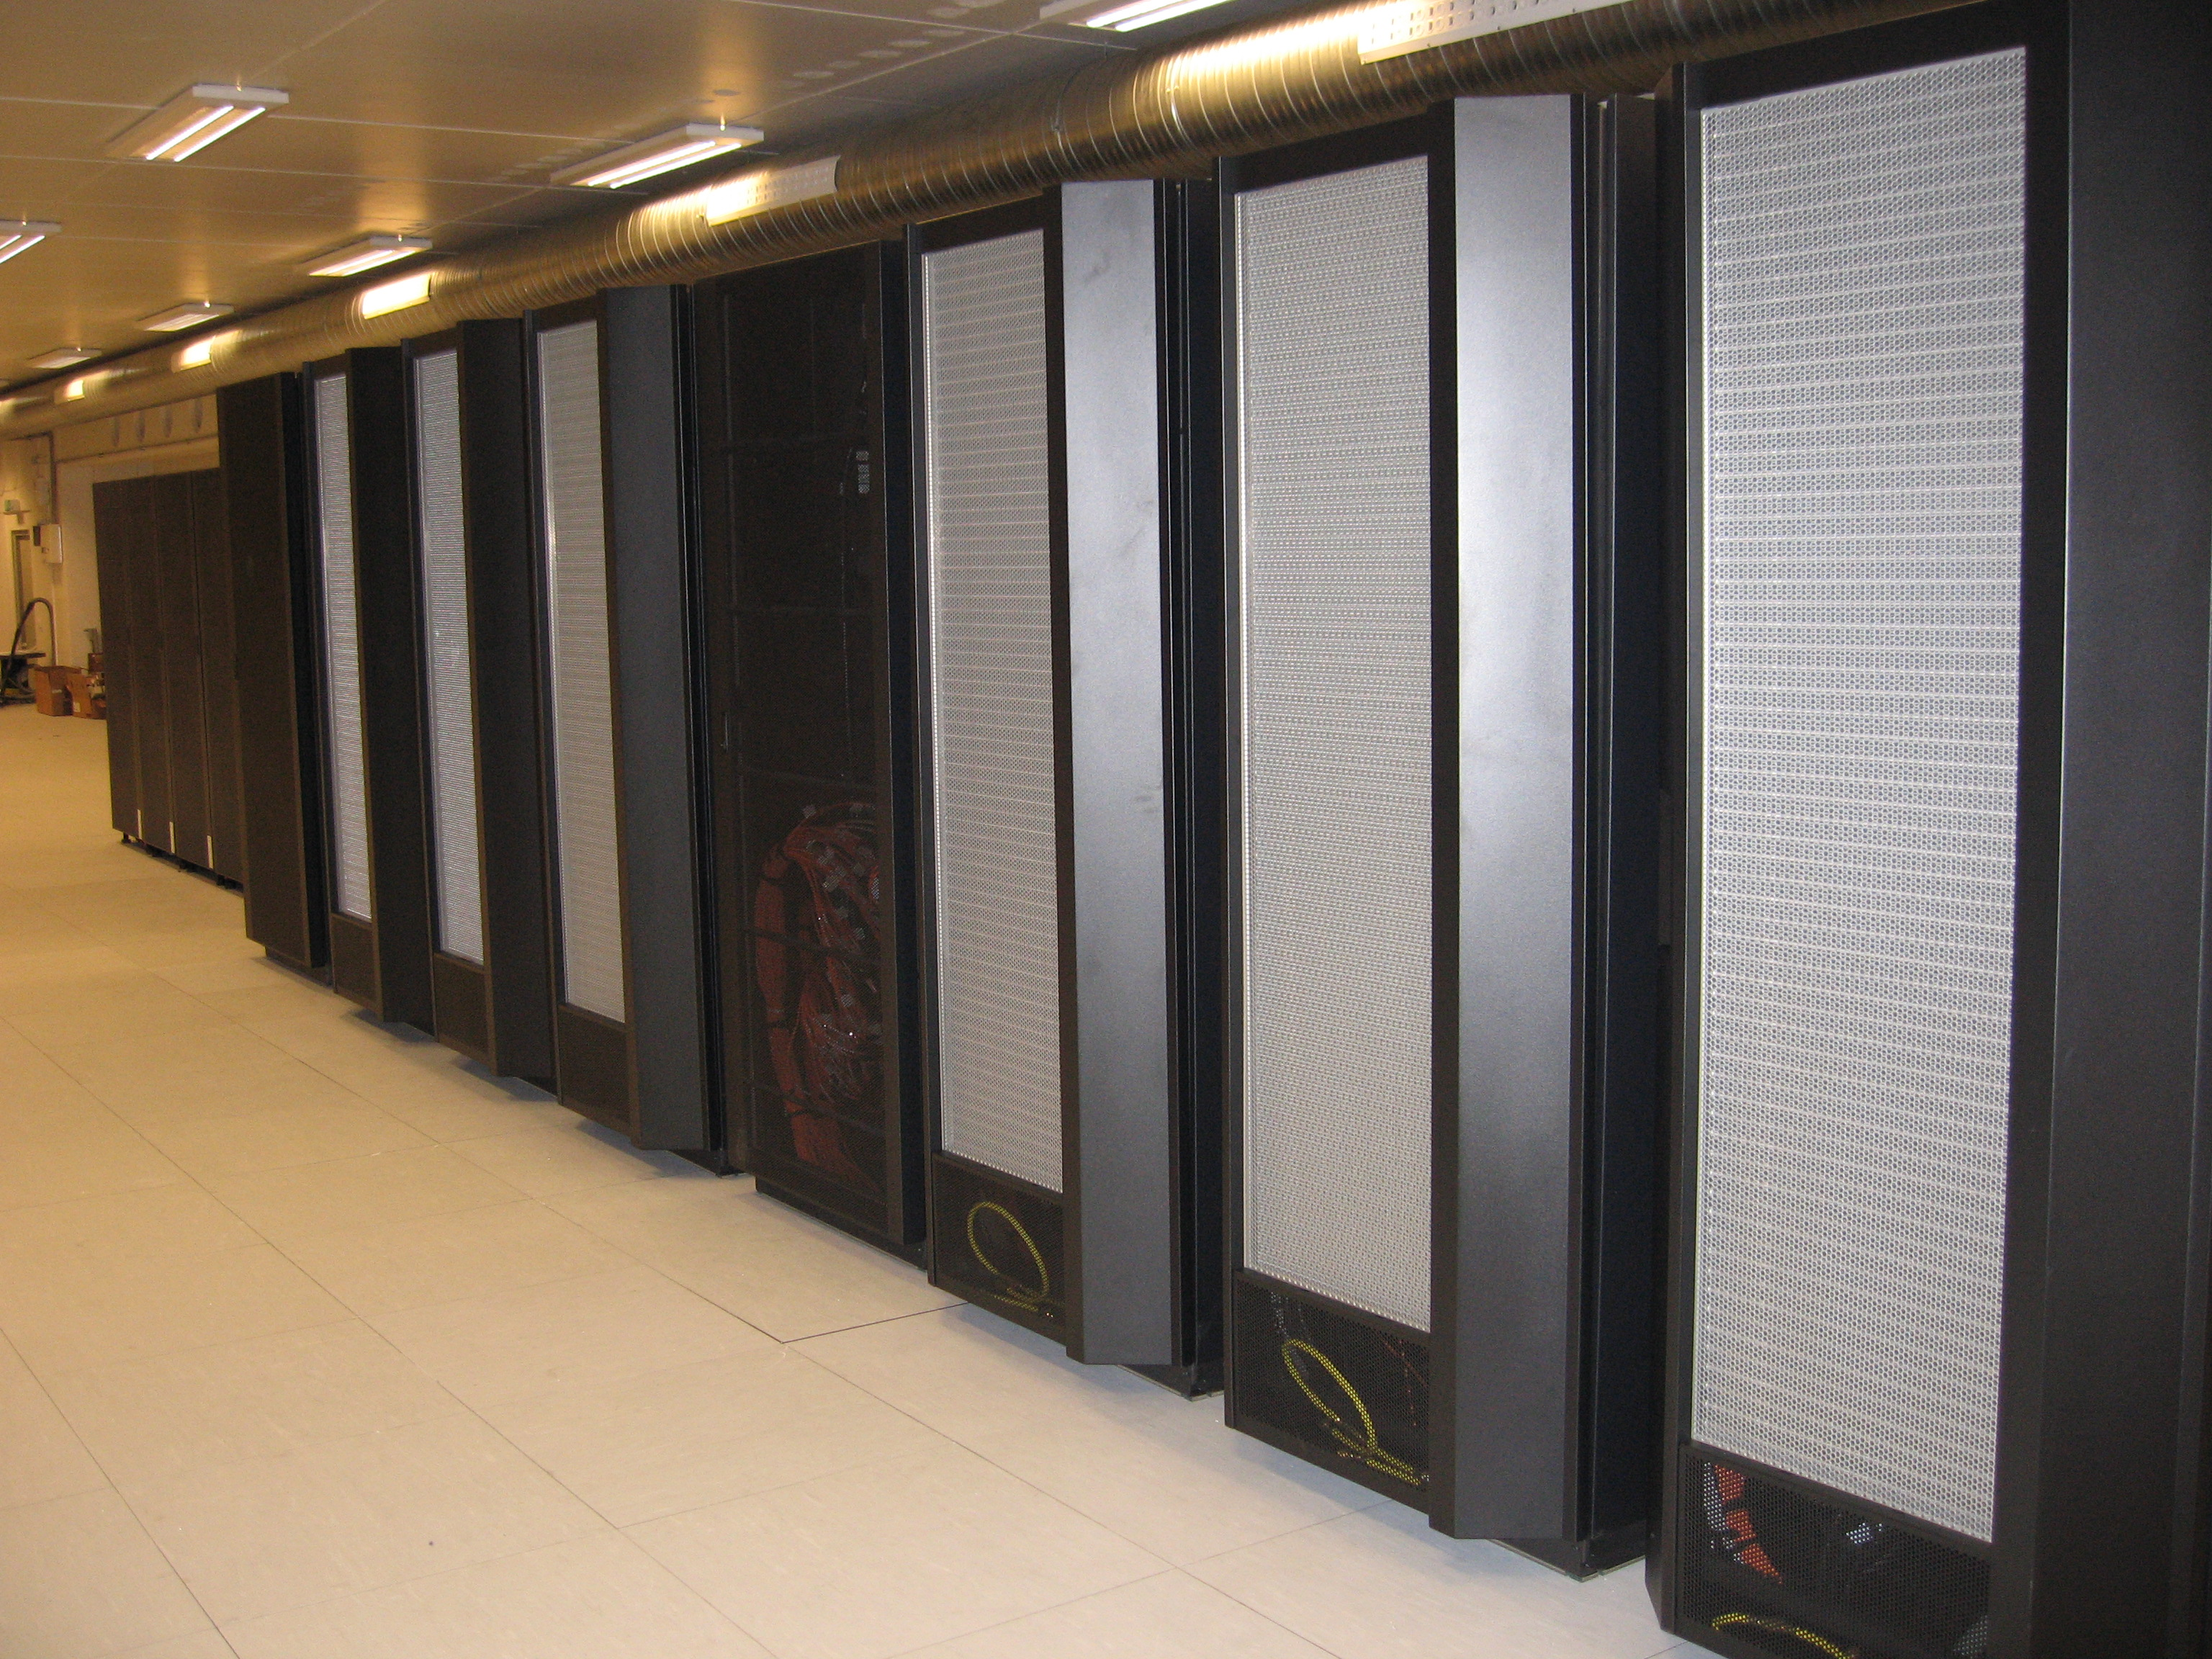
\includegraphics[width=0.6\textwidth]{njord_2}
  \caption{
    \emph{Njord}, the previous IBM supercomputer system at NTNU. Courtesy of
    Arve Dispen.
  }
  \label{fig:njord}
\end{figure}

\begin{figure}
  \centering
  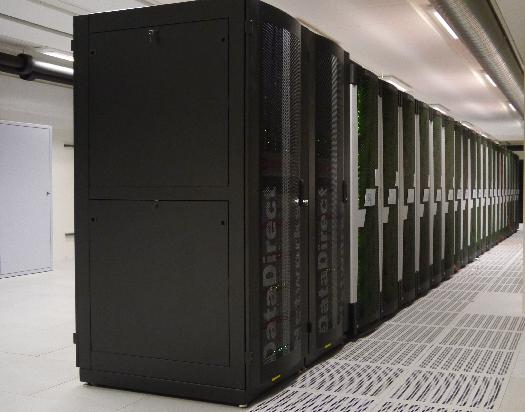
\includegraphics[width=0.6\textwidth]{vilje}
  \caption{
    Photo of \emph{Vilje}, the current SGI supercomputer at NTNU.
    Source: NTNU HPC Wiki.
  }
  \label{fig:njord}
\end{figure}

\section{Applications}

Some sample applications for supercomputing are given in \Autoref{fig:met,
fig:climate}.

\vspace{2cm}
\begin{figure}[!ht]
  \centering
  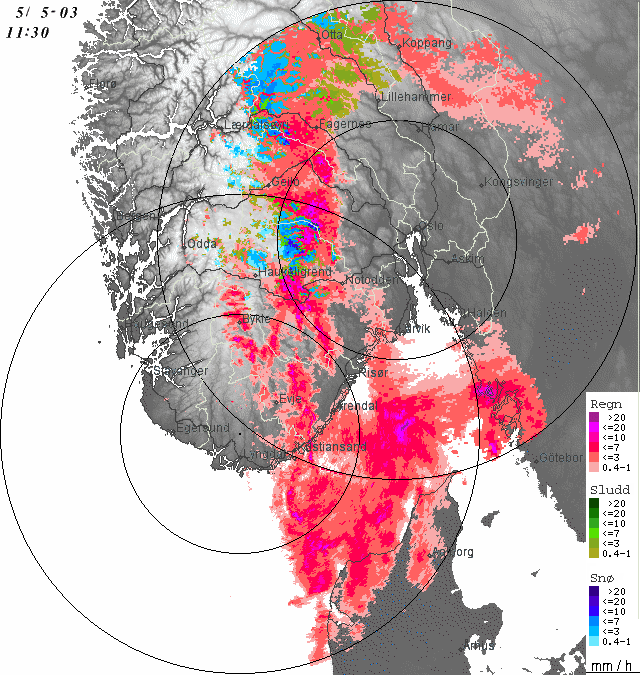
\includegraphics[height=0.6\textheight]{met}
  \caption{
    Example of use of supercomputing: weather forecasting. The Meteorological
    Institute in Norway uses the supercomputer \emph{Njord} every day. Source:
    \protect\url{http://met.no}.
  }
  \label{fig:met}
\end{figure}

\begin{figure}[!ht]
  \centering
  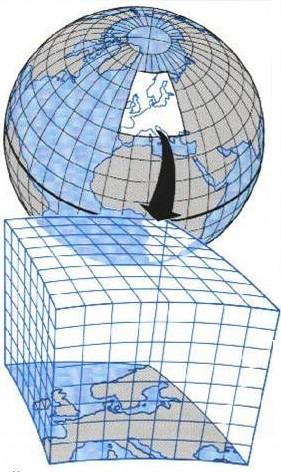
\includegraphics[height=0.6\textheight]{climate_model}
  \caption{
    Example of use of supercomputing: climate modelling. For more information,
    see \protect\url{http://bjerknes.uib.no} (Bjerknes Centre for Climate Research).
  }
  \label{fig:climate}
\end{figure}

\chapter{Single processor systems}

\section{A prototypical processor}

We start by explaining some of the basic tasks performed by a single processor.
The comments are particularly relevant for the MIPS R14000 processor used in a
previous supercomputer at NTNU (called \emph{Gridur}, a SGI Origin 3000 system
used in the period 2001--2007). The MIPS processor is an example of a processor
implementing a RISC architecture (RISC---\emph{Reduced Instruction Set
Computer}), which has been a very important processor design over the past
couple of decades. We will later return to comment on the POWER5 processor
used in the previous supercomputer at NTNU, in particular some of the key
differences compared to the processor discussed in this section. The name POWER
refers to {\em Performance Optimization With Enhanced RISC}, and is also the
name of a series of microprocessors designed by IBM.

\begin{figure}[htbp]
  \centering
  \begin{tikzpicture}[
    block/.style={
      draw=darkblue,
      fill=cadet,
      shape=rectangle,
      rounded corners=1mm,
      text height=1.5ex,
      text depth=.25ex,
    },
    l1/.style={
      minimum height=8mm,
      minimum width=4cm,
    },
    ops/.style={
      minimum height=8mm,
      minimum width=4cm,
      align=right,
    },
    inst/.style={
      minimum height=28mm,
      minimum width=16mm,
    },
    line/.style={
      thick,
      draw=darkblue,
    }]
    \node[block, l1] (L1inst) {L1 Instruction Cache};
    \node[block, l1, right=15mm of L1inst] (L1data) {L1 Data Cache};
    \node[block, l1, above=8mm of L1inst, fill=salmon] (Rest) {RAM, disk, network};
    \node[block, l1, above=8mm of L1data, fill=salmon] (L2) {L2 cache};
    \node[block, ops, below=16mm of L1data.east, anchor=east] (LS) {Load and store};
    \node[block, ops, below=10mm of LS.east, anchor=east] (Int) {Integer};
    \node[block, ops, below=10mm of Int.east, anchor=east] (Float) {Floating point};
    \node[block, inst, below=26mm of L1inst.east, anchor=east] (Decode) {Decode};
    \node[block, inst, below=26mm of L1inst.west, anchor=west] (Branch) {Branch};
    \node[block, inst, below=2mm of Decode, minimum height=8mm] (Clock) {Clock};

    \draw[line, <->] (Rest.east) -- (L2.west);
    \draw[line, <->] (L1inst.east) -- (L1data.west);
    \draw[line, <->] (L1data.south) -- (LS.north);
    \draw[line, ->] (Decode.east) -- (Int.west);
    \draw[line, ->] ([yshift=10mm]Decode.east) -- (LS.west);
    \draw[line, ->] ([yshift=-10mm]Decode.east) -- (Float.west);
    \draw[line, ->] (Decode.west) -- (Branch.east);
    \draw[line, ->] ([xshift=12mm]L1inst.south) -- (Decode.north);
    \draw[line, <-] ([xshift=-12mm]L1inst.south) -- (Branch.north);
    \draw[line] ($(L1inst.east)!0.5!(L1data.west)$) -- ($(Rest.east)!0.5!(L2.west)$);
  \end{tikzpicture}
  \caption{
    A prototypical processor, including the MIPS R14000 used in \emph{Gridur},
    the supercomputer at NTNU during the period 2001--2007. The red components
    are off-chip.
  }
  \label{fig:Lande}
\end{figure}

In order to introduce some key concepts in the RISC architecture, let us briefly
explain what happens when we perform the following simple operation
\begin{align}
  c = a + b.
  \label{single:add1}
\end{align}
Here, we want the processor to add the two numbers $a$ and $b$ and store the
answer in $c$. In this case, $a$ and $b$ are referred to as \emph{operands},
while $+$ is the \emph{operator}. Hence, the simple addition of two scalars
implies a single floating point operation.

The basic unit of ``time'' for our processor is a clock cycle. The state of the
processor changes from clock cycle to clock cycle, depending on what needs to be
done. Different parts/units of the processor work on different tasks
independently of each other. These tasks may correspond to different
instructions, each in a particular phase of completion.

Consider again the addition of two scalars. The operation \eqref{single:add1}
may be part of a larger program involving many operations (or instructions). Let
us assume that the instruction for the ``add'' operation is currently in a small
memory module denoted as L1 cache (for instructions). When the execution of our
program is ready to perform this operation, the instruction is brought into a
decoder and made ready for execution. The addresses of the operands ($a$ and
$b$) are computed and the operands are brought into two registers of the
processors. We assume that the operands are available in the small memory module
called L1 cache (for data).

The operands are then directed from the two registers to the floating point unit
for addition (denoted as FPAdd) where the two numbers are added together. The
whole operation takes just a few clock cycles. For the MIPS R14000 processor,
this operation takes five clock cycles:
\begin{enumerate}
\item read from register
\item align
\item add
\item pack
\item write to register
\end{enumerate}
Note that the number of clock cycles required to perform this operation is not
the same as the number of bits used to store our operands (e.g., 64 bits in
double precision). The reason is that the data flow in the processor happens
along a ``wide bus'' capable of moving all the bits at the same time. This is an
example of bit-level parallelism. Older processors could only move 4, 8, 16, and
32 bits at a time and an add operation therefore took additional clock cycles to
complete. In addition, current processors have a much higher clock frequency (or
shorter clock period) compared to older processors.

Let us now make a few more remarks regarding the processor in
\autoref{fig:Lande}. We have already mentioned the floating point unit for
addition, FPAdd. However, the processor has also other functional units. For
example, the R14000 prosessor has five functional units which can operate
independently from each other:
\begin{itemize}
\item Load/Store: computes memory addresses and to bring operands to and from
the memory;
\item ALU1: a unit for addition and subtraction of integers, and logical
operations;
\item ALU2: a unit for addition, subtraction, multiplication, and division of
integers, as well as logical operations;
\item FPAdd: adds of floating point numbers;
\item FPMult: a unit for multiplication, division, and square root of floating
point numbers.
\end{itemize}
Note that the operands used in these functional units need to come from the
registers in the processor. If the operands are not in the registers, they have
to be brought from the memory into the registers with a {\em load} operation.
The answer (or output) from the functional units are also stored in registers
and subsequently stored in the memory with a {\em store} operation.

\section{Memory hierarchy}

The example from the previous section involving the addition of two floating
point numbers assumed that the instruction for the operation \eqref{single:add1}
was in the memory module denoted as L1 cache for instructions; see
\autoref{fig:Lande}. Similarly, we assumed that the operands $a$ and $b$ were
available in the memory module denoted as L1 cache for data.

Let us now comment a bit more on what happens if these assumptions are not true.
In this case, the program will check whether the instruction or data are
available in the memory module denoted as L2 cache in Figure \ref{fig:Lande}.
This is a memory module which is larger than L1 cache. Furthermore, the L2 cache
is not split into a separate module for instructions and a separate module for
data. It also takes longer (meaning more clock cycles) to fetch data from L2
cache compared to L1 cache. It could also happen that the instruction and the
data the program is looking for is not available in L2 cache either. In this
case data has to be brought in from main memory (RAM) or perhaps even further
away (e.g. the local disk).

Bringing instructions and data to and from memory (from cache, RAM, etc.) is
typically a bottleneck in scientific computing. The processors are getting
faster and faster, but the memory bandwidth (or transfer rate in bytes per
second) is not keeping up at a similar speed. Hence, for certain operations, the
processor can become ``starved'' for data, meaning that it is idle for much of
the time while waiting for data to be transferred to and from memory. The
overall performance in terms of floating point operations per second will in
such cases not be governed by the processor speed, but by the memory access
time.

In order to ``hide'' this difference in speed (i.e., processor speed versus
memory access speed), the memory is organized in a hierarchical fashion;
see \autoref{fig:MemoryHierarchy}.
\begin{figure}
  \centering
  \begin{tikzpicture}[
    line/.style={
      thick,
      draw=darkblue,
    }]
    \coordinate (A) at (-4.5,0) {};
    \coordinate (B) at (4.5,0) {};
    \coordinate (C) at (0,7.4) {};
    \fill[cadet] (A) -- (B) -- (C);
    \draw[line, name path=AC] (A) -- (C);
    \draw[line, name path=BC] (B) -- (C);
    \foreach \y/\A in
    {0/Tape, 1/Distributed memory, 2/Local disk, 3/Main memory (RAM), 4/Cache, 5/Registers, 6/CPU}
    {
      \path[name path=horiz] (A|-0,\y) -- (B|-0,\y);
      \draw[line, name intersections={of=AC and horiz,by=P},
      name intersections={of=BC and horiz,by=Q}] (P) -- (Q)
      node[midway, above=1mm, text height=1.5ex, text depth=.25ex] {\A};
    }
  \end{tikzpicture}
  \caption{
    The memory hierarchy of a computer system. Higher entries are faster, while
    lower entries are cheaper and larger.
  }
  \label{fig:MemoryHierarchy}
\end{figure}
The fastest part of the memory is closest to the CPU. For example, on the MIPS
R14000, the L1 cache is on the chip. This part of the memory is fast, but also
small because it is very expensive. In contrast, the main memory is much larger,
but has also a much longer access time; see \autoref{tbl:cycles}. We will later
discuss in more detail how it is decided what should be in the L1 and L2 cache.

\begin{table}
  \centering
  \caption{
    Typical memory access times for R14000. The numbers represent number of
    clock cycles.
  }
  \label{tbl:cycles}
  \bgroup\def\arraystretch{1.2}
  \begin{tabular}{rl}
    \hline
    Memory type & Clock cycles \\ \hhline{==}
    Registers & $1$ \\ \hline
    L1 cache & $2$--$3$ \\ \hline
    L2 cache & $10$--$12$ \\ \hline
    Main memory &  $100$--$200$ \\ \hline
    Message passing & $\mathcal{O}(10^3)$--$\mathcal{O}(10^4)$ \\ \hline
    Local disk & $\mathcal{O}(10^6)$ \\ \hline
  \end{tabular}
  \egroup
\end{table}

We remark that message passing in \autoref{tbl:cycles} refers to communication
between individual processors by sending messages over a network; we will return
to a discussion of multiple processors later.

\section{Pipelining/vectorization}

Assume now that, instead of (\ref{single:add1}), we would like to add the two
vectors $\bm a$ and $\bm b$ of length $n$ and store the result in a vector $\bm
c$, i.e.
\begin{align}
  \bm c = \bm a + \bm b.
  \label{single:addn}
\end{align}
We can also write \eqref{single:addn} as the loop (in Fortran)
\begin{lstlisting}[style=fortran]
  for i=1,n
    c(i) = a(i) + b(i)
  end
\end{lstlisting}
Again, we start by assuming that the data are available in the registers. From
there, the individual vector elements $a(i)$ and $b(i)$ enter the floating point
unit FPAdd where the numbers are added to produce the output elements $c(i)$,
$i=1,\ldots,n$.

We mentioned earlier that it takes five clock cycles to add two floating point
numbers together. This would perhaps suggest that the total number of clock
cycles for the operation \eqref{single:addn} is $5n$, and that the total
execution time therefore is $5n\tau$ where $\tau$ is the clock period. However,
if things are done optimally, the total number of clock cycles can be reduced to
approximately $n$ for $n\gg 1$. The reason for this is that the five stages in
the adder correspond to independent tasks. This means that, as soon as the
addition of two operands (i.e. $a(i)$ and $b(i)$) has finished the first stage,
two new operands ($a(i+1)$ and $b(i+1)$) can enter the first stage in the adder.
Hence, after five clock cycles, the first number $c(1)$ in the operation
\eqref{single:addn} is ready, while the numbers $c(2)$, $c(3)$, $c(4)$, $c(5)$,
and $c(6)$ are in different phases of completion in the adder.

In summary, after a few clock cycles to ``fill up'' the adder, a new answer
$c(i), i=2,\ldots,n$ is ready every clock cycle. This is what is referred to as
\emph{pipelining} (or sometimes \emph{vectorization}). The reason behind this
term is quite obvious: we constantly feed the floating point unit (in this case,
the adder) so that the ``pipeline'' is always full. In other words, we do not
wait until one answer is ready before we start the process of adding two new
numbers. In this way, we achieve a certain level of parallelism in the sense
that asymptotically (for long vector lengths), the adder works simultaneously on
five different pairs of operands.

The above discussion assumed that the data (i.e. the operands $a(i)$ and $b(i)$,
$i=1,\ldots,n$) are ready for the adder with no delay. Whether this is possible
or not depends on the particular processor. In the case of the MIPS R14000
processor it is not possible to achieve this performance. The reason is that,
in the best case, only a single floating point number can be brought between the
memory (L1 cache) and a register at a time. Since we need to fetch two operands,
$a(i)$ and $b(i)$, per floating point operation, and store the answer $c(i)$
back to memory, a minimum of three clock cycles are needed for memory transfer
per addition. Hence, even though the floating point unit (the adder) can
theoretically complete one addition per clock cycle, the memory traffic will be
the bottleneck, at least for large $n$.

The only possibility for achieving a better performance is if all the operands
are already available in the processors registers. However, since a processor
only has a limited number of registers (on the MIPS R14000 the number of
registers is 64), such performance cannot be acheived if $n \gg 1$.

Let us now predict the optimal performance for the operation \eqref{single:addn}
in the case $n \gg 1$ on Gridur. The clock cycle for each processor is 500 MHz.
Hence, the clock period is 2 ns. Since each floating point operation will
asymptotically require three clock cycles due to the fetch and store operations
(see the discussion above), each floating point operation will at least require
three clock cycles, or 6 ns. Hence, the maximum performance for the operation
\eqref{single:addn} is $(6\cdot 10^{-9})^{-1}$ floating point operations per
second, or approximately 167 MFlops. In practice, less performance may be
achieved, in particular if the operands need to first be brought in from deeper
layers of the memory hierarchy; see \autoref{fig:MemoryHierarchy}.

\section{Superscalar operations}

Consider now a modification of the operation \eqref{single:addn} to the
following operation:
\begin{align}
  \bm c = \bm a + \gamma \bm b.
  \label{single:addmultn}
\end{align}
Here, each vector element $b(i)$, $i=1,\ldots,n$ is multiplied with a scalar,
$\gamma$, before being added to $a(i)$. Similar to the operation
\eqref{single:addn} the result of each addition is stored as the vector element
$c(i)$.

The new operation here is the multiplication. As mentioned earlier, each R14000
processor has a separate floating point unit for multiplication, FPMult. Similar
to the add operation, multiplying two numbers also take five clock cycles:
\begin{enumerate}
\item read from register
\item multiply
\item sum product
\item pack
\item write to register
\end{enumerate}
Hence, all the comments made in the previous section for the operation
\eqref{single:addn} also apply if the add operation $+$ is replaced by
multiplication $\times$.

Let us now comment on what happens when we combine both multiplication and
addition as in \eqref{single:addmultn}. Again, let us first assume that all the
data are readily available (i.e. stored in the registers). The vector elements
$b(i)$ are brought to the multiplier where each element is multiplied by the
scalar $\gamma$; see Figure \autoref{fig:SuperScalar}. After a startup time of
five clock cycles, a new answer is coming out from the multiplier every clock
cycle. We assume here that the pipelining feature is exploited.

\begin{figure}[htbp]
  \centering
  % \begin{center}
  %   \includegraphics[scale=0.9]{SuperScalar}
  % \end{center}
  \begin{tikzpicture}[
    block/.style={
      draw=darkblue,
      fill=cadet,
      shape=rectangle,
      rounded corners=1mm,
      minimum height=12mm,
      minimum width=12mm,
    },
    pinin/.style={pin edge={to-, thick, darkblue}},
    pinout/.style={pin edge={-to, thick, darkblue}},
    ]
    \node[block, pin={[pinin]above:$\gamma$}, pin={[pinin]left:$b(i)$}] (mult) {$\times$};
    \node[block, right=20mm of mult, pin={[pinin]above:$a(i)$}, pin={[pinout]right:$c(i)$}] (add) {$+$};
    \draw[darkblue, ->, thick] (mult.east) -- (add.west);
  \end{tikzpicture}
  \caption{The superscalar operation multiply and add.}
  \label{fig:SuperScalar}
\end{figure}

Each output from the multiplier is now channeled directly as an input to the
adder where it is added to the vector element $a(i)$. After another five clock
cycles, the answer $c(i)$ is ready. Hence, after a startup time of 10 clock
cycles (5 for the multiplier and 5 for the adder), we get one complete answer
$c(i), \, i=1,\ldots,n$ as output every clock cycle. Asymptotically (i.e., for
large vector lengths), the theoretical performance is therefore two floating
point operations per clock cycle. This way of piping the output from one
floating point unit into the input for another unit is denoted as
\emph{superscalar} capability. Similar to the pipelining feature of the adder
and the multiplier, the superscalar capability offers yet another possibility of
parallelism in the sense that each single processor is capable of performing
addition and multiplication at the same time (for sufficiently long vector
lengths).

In practice, the processor has only a limited number of registers, and we need
to fetch the operands from memory (L1 cache) and store the answers in memory.
Similar to the operation \eqref{single:addn}, each complete vector element
$c(i)$ will require three clock cycles due to the memory traffic. However, in
contrast to the operation \eqref{single:addn}, the operation
\eqref{single:addmultn} implies two floating point operations instead of one for
each complete vector element $c(i)$. The maximum single-process performance we
can obtain on R14000 for \eqref{single:addmultn} is thus twice the performance
for \eqref{single:addn}, i.e. 333 MFLOPS.

\section{Cache}

Let us now discuss in more detail the interaction between the cache and the main
memory. The main purpose of the cache is to keep copies of data in extra (and
fast) memory close to the CPU in order to ``hide'' the relatively slow transfer
rate between the main memory and the processor.

Because fast caches are expensive, they tend to be small. As an example, we give
the memory sizes for the R14000 processors. On Gridur, four individual
processors shared up to 4 Gbytes of main memory. Each processor had an L2 cache
of size 8 Mbytes and two L1 caches (one for instructions and one for data), each
only of size 32 Kbytes. Hence, the L1 cache for data can only hold up to 4000
floating point numbers (assuming double precision), which is relatively small in
the context of simulating systems with thousands or millions of unknowns (e.g.,
for the numerical solution of partial differential equations). The L2 cache can
hold more data, but the transfer rate is a little bit longer compared to the L1
cache; see \autoref{tbl:cycles}.

The cache is smaller than the main memory by some power of two. Hence, a
strategy for mapping memory locations to cache locations needs to be defined. We
describe three strategies for doing this.

\subsection{Direct mapped cache}

One strategy is to use what is refered to as a \emph{direct mapped cache}. In
this case, each location in main memory corresponds to a unique location in
cache; see \autoref{fig:DirectMappedCache}. The main memory address is split
into two parts: the first bits of the memory address are called the \emph{set
bits} and these bits give the precise cache address. The remaining bits are
called the \emph{tag bigs}, and these are used to determine if a copy of the
content at the particular main memory location has been copied into the cache
location given by the set bits. With this strategy we see that several main
memory addresses map to the same cache address.
\[
  \text{Memory address} =
  \underbrace{b_1 \ldots b_k}_{\text{tag bits}}
  \underbrace{b_{k+1} \ldots b_{N}}_{\text{cache address}}.
\]

\begin{figure}
  \centering
  \begin{tikzpicture}[scale=0.3]
    \def \n {7};
    \def \k {3};
    \def \q {1};
    \def \s {3};

    \foreach \i [
      evaluate=\i as \R using -(\n+1)*\i,
      evaluate=\i as \L using -(\n+1)*(\i+1),
    ] in {0,...,\k}
    {
      \fill[cadet] (\R-\q, 0) -- (\R-\q, -2) -- (\R-\q-1, -2) -- (\R-\q-1, 0) -- (\R-\q, 0);
      \fill[salmon] (\R-\s, 0) -- (\R-\s, -2) -- (\R-\s-1, -2) -- (\R-\s-1, 0) -- (\R-\s, 0);
      \draw[darkblue, very thick] (\R, 0) -- (\R, -2) -- (\L, -2) -- (\L, 0) -- (\R, 0);
      \foreach \j [
        evaluate=\j as \l using \R-\j
      ] in {1,...,\n}
      {
        \draw[darkblue, very thin] (\l, 0) -- (\l, -2);
      }
    }

    \fill[cadet] (-\q, 3) -- (-\q, 1) -- (-\q-1, 1) -- (-\q-1, 3) -- (-\q, 3);
    \fill[salmon] (-\s, 3) -- (-\s, 1) -- (-\s-1, 1) -- (-\s-1, 3) -- (-\s, 3);
    \draw[darkblue, very thick] (0, 3) -- (0, 1) -- (-\n-1, 1) -- (-\n-1, 3) -- (0, 3);
    \foreach \j in {1,...,\n} {
      \draw[darkblue, very thin] (0-\j, 3) -- (0-\j, 1);
    }

    \node[anchor=west] at (0, -1) {RAM};
    \node[anchor=west] at (0, 2) {Cache};
  \end{tikzpicture}
  \caption{
    A direct mapped cache. Each main memory address maps to a unique and
    pre-determined location in the cache.
  }
  \label{fig:DirectMappedCache}
\end{figure}

When some particular data is requested by the program, e.g., a floating point
number, the processor will check whether the data is stored in L1 cache. It does
this by looking up the cache address (taking the least significant bits of the
memory address) and checking whether the tag bits at that location match the tag
bits of the memory address. If is not in L1 cache, the processor will check
whether the data is stored in L2 cache. If this is the case, the requested data
will be copied from the L2 cache into L1 cache. If the data is not in L2 cache
either, the data will have to be brought in from main memory. In this case, a
copy will be made in L2 cache as well as in L1 cache. In either case, the tag
bits at the given cache address will be updated to match the new mapped
location.

Note that when a floating point number (or an integer) is requested by the
program, more than a single number is copied into cache. The minimum amount of
data copied is called a {\em cache line}. For the R14000 processor, the cache
line for the L1 cache is 32 bytes (corresponding to four floating point numbers
in double precision), while the cache line for the L2 cache is 128 bytes
(corresponding to 16 floating point numbers in double precision). The extra
numbers copied are the numbers in the adjacent memory locations in main memory.

Consider again the operation \eqref{single:addn}. Assume that the vectors $\bm
a$, $\bm b$ and $\bm c$ represent floating point numbers in double precision,
and that the vectors are stored after each other in main memory. Let the vector
length $n=4000$, i.e. each vector will precisely fill the L1 data cache. For
every element $c(i)$ computed, the operands $a(i)$ and $b(i)$ will need to be
brought in all the way from main memory due to the fact that $a(i)$, $b(i)$ and
$c(i)$ happen to have the same cache address. A severe drop in performance will
be observed in this case. This situation is refered to as cache trashing; see
\autoref{fig:CacheTrashing}.

\begin{figure}
  \centering
  \begin{tikzpicture}[scale=0.3]
    \def \n {7};
    \def \k {3};
    \def \q {1};

    \foreach \i [
      evaluate=\i as \R using -(\n+1)*\i,
      evaluate=\i as \L using -(\n+1)*(\i+1),
    ] in {0,...,\k}
    {
      \fill[cadet] (\R-\q, 0) -- (\R-\q, -2) -- (\R-\q-1, -2) -- (\R-\q-1, 0) -- (\R-\q, 0);
      \draw[darkblue, very thick] (\R, 0) -- (\R, -2) -- (\L, -2) -- (\L, 0) -- (\R, 0);
      \foreach \j [
        evaluate=\j as \l using \R-\j
      ] in {1,...,\n}
      {
        \draw[darkblue, very thin] (\l, 0) -- (\l, -2);
      }
    }

    \fill[cadet] (-\q, 3) -- (-\q, 1) -- (-\q-1, 1) -- (-\q-1, 3) -- (-\q, 3);
    \draw[darkblue, very thick] (0, 3) -- (0, 1) -- (-\n-1, 1) -- (-\n-1, 3) -- (0, 3);
    \foreach \j in {1,...,\n} {
      \draw[darkblue, very thin] (0-\j, 3) -- (0-\j, 1);
    }

    \node[anchor=west] at (0, -1) {RAM};
    \node[anchor=west] at (0, 2) {Cache};
    \node[anchor=north] at (-\q-0.5, -2) {\scriptsize $a(i)$};
    \node[anchor=north] at (-\n-1-\q-0.5, -2) {\scriptsize $b(i)$};
    \node[anchor=north] at (-\n-\n-2-\q-0.5, -2) {\scriptsize $c(i)$};
    \node[anchor=south] at (-\q-0.5, 3) {\scriptsize ??};
  \end{tikzpicture}
  \caption{
    Cache trashing. The corresponding elements in the vectors $\bm a$, $\bm b$
    and $\bm c$ all map to the same cache address.
  }
  \label{fig:CacheTrashing}
\end{figure}

Cache trashing can be avoided by storing the elements in the vectors $\bm a$,
$\bm b$ and $\bm c$ in a different way; see Figure \ref{fig:AdjacentMemory}. We
remark that the crash trashing example given here is perhaps not likely to
happen. Nonetheless, it illustrates the point that severe performance
degradation is possible to observe due to undesirable memory traffic.

\begin{figure}
  \centering
  \begin{tikzpicture}[
    scale=0.8,
    every node/.style={
      text height=1.5ex,
      text depth=.25ex,
    }
    ]
    \draw[darkblue, very thick] (-6, 0) -- (6, 0);
    \draw[darkblue, very thick] (-6, 1) -- (6, 1);
    \draw[darkblue, very thin] (-3, 0) -- (-3, 1);
    \draw[darkblue, very thin] (-2, 0) -- (-2, 1);
    \draw[darkblue, very thin] (-1, 0) -- (-1, 1);
    \draw[darkblue, very thin] (0, 0) -- (0, 1);
    \draw[darkblue, very thin] (1, 0) -- (1, 1);
    \draw[darkblue, very thin] (2, 0) -- (2, 1);
    \draw[darkblue, very thin] (3, 0) -- (3, 1);
    \node at (-3.5, 0.5) {\footnotesize $\cdots$};
    \node at (-2.5, 0.5) {\footnotesize $a_i$};
    \node at (-1.5, 0.5) {\footnotesize $b_i$};
    \node at (-0.5, 0.5) {\footnotesize $c_i$};
    \node at (0.5, 0.5) {\footnotesize $a_{i+1}$};
    \node at (1.5, 0.5) {\footnotesize $b_{i+1}$};
    \node at (2.5, 0.5) {\footnotesize $c_{i+1}$};
    \node at (3.5, 0.5) {\footnotesize $\cdots$};
  \end{tikzpicture}
  \caption{Adjacent memory layout.}
  \label{fig:AdjacentMemory}
\end{figure}

\subsection{Fully associative cache}

To avoid the possibility of cache trashing, we can use a different cache
strategy called a \emph{fully associative cache}. In a fully associative cache,
each cache address can map to any memory address. This is essentially a direct
mapped cache where all the bits are used as tag bits and no bits are used as a
cache address.

To find the corresponding cache location for a given memory address, the tag
bits of all cache locations must be checked. This is typically done in parallel
using dedicated hardware, which is rather complicated. For this reason, fully
associative caches are rarely seen.

When the cache is full, a cache line must be evicted to make way for new data.
How this happens depends on the replacement policy:
\begin{itemize}
\item Least recently used (LRU);
\item Least frequently used (LFU);
\item Random
\end{itemize}
In the context of numerical solution of partial differential equations, the
alternative \emph{LRU} generally gives the best performance. This can be
understood by the fact that such problems typically exhibit significant locality
in time and space: data that has recently been used has a high chance of being
used again in the near future; and data close (in space) to recently used data
has a high chance of being used in the near future.

\subsection{Set-associative cache}

A \emph{set-associative} cache is a nice compromise between a direct mapped
cache and a fully associative cache. In a set-associative cache, the cache is
split into chunks of $n$ cache lines. Each memory address maps deterministically
to a given chunk (according to its least significant bits) precisely as a direct
mapped cache. However, within this chunk the mapping proceeds as with a fully
associative cache with $n$ choices.

The cache eviction strategies work the same way as for a fully associative
cache.

\chapter{Introduction to git}

The scope of this chapter is to explain the basic mechanisms of git. Git is a
complex tool, using it to its full power can take quite some time to learn.
Something crucial may have been missed while attempting to boil it down to
basics. There is a whole internet full of guides out there and you are
encouraged to supplement these ramblings with more verbose tutorials and
articles. Also, please do not hesitate to ask during lectures or breaks; I love
it when people talk git to me.

\section{Installing git}

Start by installing git on your laptop; on Ubuntu you can do this through
\begin{lstlisting}[style=shell]
  sudo apt-get install git
\end{lstlisting}

\section{Setting up a GIT repository}

You can set up a GIT directory in two ways. You either clone a remote repository
or initialize a new, empty one. In either case you end up on a \emph{branch}
called \emph{master} by default.

To clone a remote repository do
\begin{lstlisting}[style=shell]
  git clone <url>
\end{lstlisting}
where \texttt{<url>} is the URL of the repository to clone. E.g.
\begin{lstlisting}[style=shell]
  git clone /some/path/on/my/computer
  git clone https://github.com/TheBB/TMA4280
\end{lstlisting}
To initialize an empty repository, change to the directory you would like to use
and do
\begin{lstlisting}[style=shell]
  git init .
\end{lstlisting}

\section{Layout of a git repository}

A repository has two parts; the repository information and your local working
tree. The first contains information about all the individual commits, commit
messages, and branches (a sequence of commits) that is recorded. This is stored
in a folder called \texttt{.git} in the root of the repository. The second part
is your local copy of the files in the repository.

You can make a \emph{bare} clone of a repository. This is a directory that only
contains the repository information, i.e. only the \emph{.git} folder of a
normal clone, and no local working tree. You do this through
\begin{lstlisting}[style=shell]
  git clone --bare <url>
  git init --bare .
\end{lstlisting}

As far as git is concerned, adding files already existing locally is handled as
a change to the file where everything was changed (see further down). You just
want to add source code, not files generated by the build system or the compiler
such as object files, libraries, executables or scripts.

\section{Keeping track of changes}

You can see what changes you have made to your local working directory through
\begin{lstlisting}[style=shell]
  git diff
\end{lstlisting}
If you just want to see which files, are changed, but not the changes
themselves, you can use
\begin{lstlisting}[style=shell]
  git status
\end{lstlisting}
This is in general quite useful, it can show more things such as which changes
are marked for committing.

To mark some changes for committing, do
\begin{lstlisting}[style=shell]
  git add <file>
\end{lstlisting}
This \emph{stages} the changes, but they have not yet been committed. To commit
all staged changes, use
\begin{lstlisting}[style=shell]
  git commit
\end{lstlisting}
This will open a text editor where you can enter a commit message. You can
control \emph{which} editor by adding a line such as
\begin{lstlisting}[style=shell]
  export EDITOR=<myeditor>
\end{lstlisting}
to your \texttt{\textasciitilde/.bashrc} file if you are using bash.
Alternatively, you can specify the commit message directly.
\begin{lstlisting}[style=shell]
  git commit -m "my message"
\end{lstlisting}
You can quickly commit all changes (even unstaged ones) to all tracked files by
doing
\begin{lstlisting}[style=shell]
  git commit -a
\end{lstlisting}
The two can be combined:
\begin{lstlisting}[style=shell]
  git commit -am "my message"
\end{lstlisting}

\section{Keeping track of commits}
You can see the commit log through
\begin{lstlisting}[style=shell]
  git log
\end{lstlisting}
You can see the log of commits through
\begin{lstlisting}[style=shell]
  git show <commit>
\end{lstlisting}
The commit hash can be found using git log. Alternatively, you have a few
shortcuts. If you omit the revision, the last commit in the branch will be
shown. If you want to show the previous commit, you can use
\begin{lstlisting}[style=shell]
  git show HEAD~1
\end{lstlisting}

\section{Working with remote repositories}
A remote repository is a clone of this repository. Since GIT is a distributed
revision control system, you can clone a clone, and it still contains all the
information the original clone had.

To add a new remote repository, use
\begin{lstlisting}[style=shell]
  git remote add <name> <url>
\end{lstlisting}
where \texttt{<name>} is a name you want to give the remote. If you initialize a
repository through cloning another, the repository you cloned will be registered
as a remote named \emph{origin}. If you started from scratch, there will be no
remotes by default.

To send data between remotes you can \emph{push} or \emph{pull}.

To push changes to a remote, use
\begin{lstlisting}[style=shell]
  git push <remote> <branch>
\end{lstlisting}
If you omit the branch name, all branches will be pushed. If changes you have
done conflict with changes done in the remote GIT, your push will be denied. You
then have to \emph{pull} from the remote before you push. A push will also be
denied if you push to a remote with a local working tree, and you try to push to
the branch currently checked out on the remote.

To pull changes from a remote, use
\begin{lstlisting}[style=shell]
  git pull --rebase <remote> <branch>
\end{lstlisting}
If you omit the branch name, all branches will be pulled. Please do not forget
the rebase, or you can get yourself in trouble. The pull model is more involved
to explain, and deemed outside the scope of this document.

If there are conflicts, git will try to resolve them. If it cannot, you must do
it. To see which files are in conflict you can use \emph{git status}. Where
there were conflicts you will have something that looks like the following:
\begin{lstlisting}
  <<<<<<< HEAD
  line11
  line22
  =======
  line12
  line21
  >>>>>>> 7f8de8cd5f58cd2fa0b2d18f002ce9d9431c0b8c
\end{lstlisting}

The first line is a starting marker. This is followed by lines that are in
conflict, these are from the local repository. After the equal signs follow the
lines in conflict from the remote repository. Finally an ending marker and the
commit hash from the remote. Change it into what you want it to be and save the
file. Remember that there may be multiple blocks in conflict in each file!

Stage the resolved files through \texttt{git add} and continue the rebase by
doing
\begin{lstlisting}
  git rebase --continue
\end{lstlisting}

\chapter{Multiprocessor systems}

\section{Supercomputing}

Supercomputing represents the high performance segment of the overall computing
market. This segment has traditionally been driven by grand challenge problems
in science and engineering. This is still the situation, although new areas and
new applications are constantly being added to the list of problems where
supercomputing is necessary (or at least highly desirable).

A strong motivation for using supercomputing is the possibility of performing
larger and more realistic simulations, e.g., by solving more detailed
mathematical models in science and engineering. Hence, the design of the largest
computing systems have traditionally be driven by challenges in science and
engineering.

About 30--40 years ago, supercomputers were typically specially designed vector
processors capable of performing operations on vector data. A single instruction
could operate on multiple data elements (vectors) at once, and the hardware
comprised custom-made chips. Because of the low production volume and the costly
development effort, each supercomputer was very expensive.

Supercomputers in the 80s and 90s also used fast, expensive, custom-made chips,
and combined a few of these in a multiprocess context. However, starting in the
late 80s, microprocessor-based supercomputers became more and more popular.
These systems were also called \emph{massively parallel processors} (MPPs)
because they used many more processors than traditional vector supercomputers.
The advantage of the microprocessor-based supercomputers was the use of
standard, off-the-shelf microprocessors instead of using costly, custom-made
chips. The supercomputer market today is dominated by MPP systems. A
supercomputer system typically combines thousands of processors. Some of the
largest systems comprise hundreds of thousands of processors.

Supercomputing is very resource demanding in terms of floating point operations,
memory and storage requirement, as well as visualization capabilities. Thus,
some of the important challenges related to the development and use of a
multiprocessor system concern:
\begin{enumerate}
\item communication between the processors \\
(network topology, memory access, programming models);
\item development of suitable computational methods or algorithms \\
(e.g., domain decomposition algorithms);
\item scalability (both in terms of hardware and algorithms);
\item handling of large volumes of data (storage and visualization).
\end{enumerate}

We add some additional remarks regarding scalability. Let $T_P$ be the time to
solve a given problem on $P$ processors, where time refers to wall clock time.
We define the speedup, $S_P$, as
\begin{align}
  S_P = \frac{T_1}{T_P},
  \label{multi:speedup}
\end{align}
i.e. as the ratio between the solution time on a single processor divided by the
solution time on $P$ processors. Ideally, we would like $S_P$ to be equal to
$P$, implying the $P$ processors should be able to solve the problem $P$ times
as fast as a single processor. A more realistic situation is depicted in
\autoref{fig:scalability}: for small systems (i.e. when $P$ is small), we
typically get good speedup for a fixed problem. As more processors are added,
the computational task per processor is reduced, while the communication
overhead between the processors typically increases. Hence, after a certain
number of processors, it does not pay off to add more processors.

Note that the above situation gives a too pessimistic view of supercomputing.
The assumption about a fixed problem size is typically not correct. With the
availability of larger computing systems, the problem size is typically also
increased. Many problems solved on large systems are of a size that cannot be
solved in a single processor context, either because of the storage requirement,
because of the computational cost, or both. From this view point, the definition
of speedup in \eqref{multi:speedup} must be used with some care.

\begin{figure}
  \centering
  \begin{tikzpicture}
    \begin{axis}[
      xmin=0,
      xmax=1.3,
      ymin=0,
      ymax=1.3,
      axis lines=middle,
      ticks=none,
      xlabel={$P$},
      ylabel={$S_P$},
      ]
      \addplot[dashed, thick, domain=0:1.1, samples=100]{x};
      \addplot[blue, thick, domain=0:1.3, samples=100]{x/(1+x^5)};
      \node at (axis cs:1.0,1.1) [anchor=east] {Ideally};
      \node at (axis cs:1.13,0.3) [anchor=east] {Realistically};
    \end{axis}
  \end{tikzpicture}
  \caption{Ideal speedup ($S_P = P$) and realistic speedup.}
  \label{fig:scalability}
\end{figure}

Finally, a couple of important reminders: when working in a multiprocessor
environment, the single-processor performance is still of utmost importance. In
particular we recall some of the possibilities of parallelism within a single
processor: bit-level, instruction-level, pipelining, and superscalar
capabilities (or multiple floating point units).

\section{Organization of multiprocessor systems}

According to Almasi and Gottlieb (1989), a parallel computer is a collection of
processing elements which communicate and cooperate to solve a problem fast.
This definition raises some immediate questions:
\begin{itemize}
\item How many processing elements should we use?
\item How should the processing elements communicate?
\item Will the parallel computer be scalable?
\item How powerful should a processor be?
\item What about programming?
\end{itemize}

\Autoref{fig:multiprocess1, fig:multiprocess2} show two examples of
organizations. In \autoref{fig:multiprocess1} each processor has a local cache
and can access memory modules via some type of interconnect. In this case, all
the memory modules can be accessed directly by all the processors. This
organization is referred to as \emph{global} or \emph{shared memory access}. In
\autoref{fig:multiprocess2} each processor has local memory and can only access
information in other memory modules via an interconnecting network. This
organization is referred to as \emph{distributed memory access}. Each
organization has its strengths and weaknesses. We will return to some of these
issues later.

\begin{figure}
  \centering
  \begin{tikzpicture}[scale=0.5]
    \foreach \i in {0,4,8}
    {
      \draw[darkblue, fill=cadet, thick] (\i,10) rectangle (\i+2,7);
      \draw[darkblue, very thin, dashed] (\i,8.5) -- (\i+2,8.5);
      \draw[darkblue, fill=cadet, thick] (\i,3) rectangle (\i+2,1.5);
      \draw[darkblue, thick] (\i+1,7) -- (\i+1,6);
      \draw[darkblue, thick] (\i+1,3) -- (\i+1,4);
      \node at (\i+1,9.25) {P};
      \node at (\i+1,7.75) {\$};
      \node at (\i+1,2.25) {M};
    }
    \draw[darkblue, thick] (0,6) rectangle (10,4);
    \node at (5,5) {Interconnect};
  \end{tikzpicture}
  \caption{A parallel computer with global memory access.}
  \label{fig:multiprocess1}
\end{figure}

\begin{figure}
  \centering
  \begin{tikzpicture}[scale=0.5]
    \foreach \i in {0,4,8}
    {
      \draw[darkblue, fill=cadet, thick] (\i,10) rectangle (\i+2,7);
      \draw[darkblue, very thin, dashed] (\i,8.5) -- (\i+2,8.5);
      \draw[darkblue, fill=cadet, thick] (\i,6) rectangle (\i+2,4.5);
      \draw[darkblue, thick] (\i+1,7) -- (\i+1,6);
      \draw[darkblue, thick] (\i+1,3.5) -- (\i+1,4.5);
      \node at (\i+1,9.25) {P};
      \node at (\i+1,7.75) {\$};
      \node at (\i+1,5.25) {M};
    }
    \draw[darkblue, thick] (0,1.5) rectangle (10,3.5);
    \node at (5,2.5) {Interconnect};
  \end{tikzpicture}
  \caption{A parallel computer with distributed memory access.}
  \label{fig:multiprocess2}
\end{figure}

\subsection{Uniform memory access}

There are several ways to achieve global memory access. One type of systems is
referred to as SMP: \emph{Symmetric Multi-Processor}. This is a configuration
where all the memory locations are ``equidistant'' in the sense that the memory
access time is the same.

An example of an SMP is a bus-based organization; see
\autoref{fig:bus_organization}. This system has a broadcast interconnect similar
to ethernet. It is inexpensive and it is easy to add processors. The
disadvantage with a bus organization is the very limited scalability, which is
due to the fact that the aggregate bandwidth is fixed. The use of caches could
potentially alleviate some of this problem, but then the question of how to
achieve cache coherency (or consistency) arises.

\begin{figure}
  \centering
  \begin{tikzpicture}[scale=0.5]
    \foreach \i in {-1,3}
    {
      \draw[darkblue, fill=cadet, thick] (\i,4) rectangle (\i+2,1);
      \draw[darkblue, very thin, dashed] (\i,2.5) -- (\i+2,2.5);
      \draw[darkblue, thick] (\i+1,1) -- (\i+1,0);
      \node at (\i+1,3.25) {P};
      \node at (\i+1,1.75) {\$};
    }
    \foreach \i in {7,11}
    {
      \draw[darkblue, fill=cadet, thick] (\i,2.5) rectangle (\i+2,1);
      \draw[darkblue, thick] (\i+1,1) -- (\i+1,0);
      \node at (\i+1,1.75) {I/O};
    }
    \foreach \i in {1,5,9}
    {
      \draw[darkblue, fill=cadet, thick] (\i,-2.5) rectangle (\i+2,-1);
      \draw[darkblue, thick] (\i+1,-1) -- (\i+1,0);
      \node at (\i+1,-1.75) {M};
    }
    \draw[red, very thick, <->] (-3,0) -- (15,0);
  \end{tikzpicture}
  \caption{
    A bus-based organization. The global memory is accessible to each processor.
  }
  \label{fig:bus_organization}
\end{figure}

Another example of an SMP is a crossbar or a switch-based organization. Similar
to a bus-based system, cache coherency is needed (e.g. via broadcast). A
crossbar has a better scalability than a bus organization. The aggregate
bandwidth is increased, but adding a processor becomes more and more expensive
as the system size grows (because the number of parts increases).

\begin{figure}
  \centering
  \begin{tikzpicture}[scale=0.5]
    \foreach \i in {0,3,6,9}
    {
      \draw[red, very thick] (0,\i) -- (11,\i);
      \draw[red, very thick] (\i,0) -- (\i,11);

      \draw[darkblue, fill=cadet, thick] (11,\i+.75) rectangle (13,\i-.75);
      \node at (12,\i) {M};
    }

    \foreach \i in {0,3}
    {
      \draw[darkblue, fill=cadet, thick] (\i-1,14) rectangle (\i+1,11);
      \draw[darkblue, very thin, dashed] (\i-1,12.5) -- (\i+1,12.5);
      \node at (\i,13.25) {P};
      \node at (\i,11.75) {\$};
    }

    \foreach \i in {6,9}
    {
      \draw[darkblue, fill=cadet, thick] (\i-1,12.5) rectangle (\i+1,11);
      \node at (\i,11.75) {I/O};
    }
  \end{tikzpicture}
  \caption{
    A crossbar interconnect. The global memory is accessible to each processor.
  }
  \label{fig:crossbar}
\end{figure}

In summary, there is a scalability problem with the interconnect both with a bus
organization and with a crossbar. In the case of the bus, the scalability issue
is due to the fixed aggregate bandwidth; in the case of the crossbar, the
scalability relates to the cost. An example of a compromise between these two
issues is the multistage interconnect; see
\autoref{fig:multistage_interconnect}.

\begin{figure}
  \centering
  \begin{tikzpicture}[scale=0.5]
    \foreach \i in {0,4,8,12}
    {
      \draw[darkblue, fill=cadet, thick] (\i-1,0) rectangle (\i+1,1.5);
      \draw[darkblue, thick] (\i,1.5) -- (\i,2.5);
      \draw[darkblue, thick] (\i,8.5) -- (\i,9.5);
      \node at (\i,0.75) {M};
    }

    \foreach \i in {0,4}
    {
      \draw[darkblue, fill=cadet, thick] (\i-1,12.5) rectangle (\i+1,9.5);
      \draw[darkblue, very thin, dashed] (\i-1,11) -- (\i+1,11);
      \node at (\i,11.75) {P};
      \node at (\i,10.25) {\$};
    }

    \foreach \i in {8, 12}
    {
      \draw[darkblue, fill=cadet, thick] (\i-1,9.5) rectangle (\i+1,11);
      \node at (\i,10.25) {I/O};
    }

    \foreach \i in {2, 10}
    {
      \foreach \j in {3.5, 7.5}
      {
        \draw[darkblue, thick] (\i-3,\j-1) rectangle (\i+3,\j+1);
        \node at (\i,\j) {Interconnect};
      }
    }

    \draw[darkblue, thick] (0,4.5) -- (0,6.5);
    \draw[darkblue, thick] (12,4.5) -- (12,6.5);
    \draw[darkblue, thick] (4,4.5) -- (8,6.5);
    \draw[darkblue, thick] (8,4.5) -- (4,6.5);
  \end{tikzpicture}
  \caption{
    A multi-stage interconnect. The global memory is accessible to each processor.
  }
  \label{fig:multistage_interconnect}
\end{figure}

\subsection{Non-uniform memory access}

An alternative to an SMP-organization is a NUMA-organization (\emph{Non-Uniform
Memory Access}); see \autoref{fig:NUMA}. The last supercomputers at NTNU all
represent examples of this type of organization.

\begin{figure}
  \centering
  \begin{tikzpicture}[scale=0.5]
    \foreach \i in {3, 10}
    {
      \draw[darkblue, thick] (\i+1,-2) -- (\i+1,0);
      \draw[darkblue, thick] (\i,-2) -- (\i+2,-2);

      \draw[darkblue, fill=cadet, thick] (\i-2,-2.75) rectangle (\i,-1.25);
      \node at (\i-1,-2) {M};

      \draw[darkblue, fill=cadet, thick] (\i+2,-1.25) rectangle (\i+4,-4.25);
      \draw[darkblue, very thin, dashed] (\i+2,-2.75) -- (\i+4,-2.75);
      \node at (\i+3,-2) {\$};
      \node at (\i+3,-3.5) {P};
    }

    \draw[red, very thick, <->] (0,0) -- (18,0);
    \node[anchor=south] at (9,0) {Scalable network};
    \node[anchor=west] at (15,-2) {$\cdots$};
  \end{tikzpicture}
  \caption{A NUMA organization.}
  \label{fig:NUMA}
\end{figure}

The Cray T3E had caches which were only used to hold data and instructions from
local memory. The computer had no mechanism to keep the caches consistent with
the global address space. The computer was an example of a non-coherent shared
memory machine. In principle, any processor could read/write from/to any memory
location in the global address space. In practice, however, messages were used
to transfer data from one local memory module to another. The programming model
was thus based on message passing. We will return to this model later.

On the SGI Origin, data from any memory location could be replicated into any of
the caches. Hardware support existed to keep the caches consistent. This is also
referred to as a ccNUMA organization (\emph{cache coherent Non-Uniform Memory
Access}). Any processor could read/write from/to any memory location. This
feature could be exploited in a shared memory programming model. However, note
that a message passing programming model could still be used on the SGI. We will
return to a discussion of the current supercomputer at NTNU later.

\subsection{Distributed memory access}

An example of a distributed memory organization is the mesh interconnect as
depicted in \autoref{fig:2Dmesh}. Each processor can access its own local memory
similar to the single processor case. However, data from the local memory
associated with the neighboring processors are obtained by message passing. The
two first bits of the message are used to determine in which direction (North,
South, East, West) to move. The two bits are then stripped off, and the message
proceeds to the next step on the two-dimensional mesh. The message itself is
trailing behind while the connection is being established. This approach is
referred to as \emph{wormhole routing} and was developed by William Dally at
MIT. The mesh interconnect was used on the Intel Paragon and the Intel Delta
supercomputers (in the 90s).

\begin{figure}
  \centering
  \begin{tikzpicture}
    \foreach \i in {0,...,3} {
      \draw[very thick, red] (\i,0) -- (\i,3);
      \draw[very thick, red] (0,\i) -- (3,\i);
    }
    \foreach \i in {0,...,3} {
      \foreach \j in {0,...,3} {
        \draw[thick, darkblue, fill=cadet] (\i,\j) circle (0.1);
      }
    }
  \end{tikzpicture}
  \caption{
    A 2D mesh interconnect. Each circle represents a processing element: a CPU,
    local cache, and a local memory, i.e., a single processor. Such a processing
    element is also referred to as a node.
  }
  \label{fig:2Dmesh}
\end{figure}

An improved version of the mesh interconnect is the 2D toroid; see
\autoref{fig:2Dtoroid}. Compared to the 2D mesh, there are wrap-around
connections in each spatial direction (horizontally and vertically) in order to
reduce the worst-case hop count.

Further extensions of the mesh interconnect are the 3D mesh or 3D toroid network
topology (e.g. used on the Cray T3D and Cray T3E supercomputers).

\begin{figure}
  \centering
  \begin{tikzpicture}
    \foreach \i in {0,...,3} {
      \draw[very thick, red] (\i,0) -- (\i,3);
      \draw[very thick, red] (0,\i) -- (3,\i);
    }
    \foreach \i in {0,...,3} {
      \draw[thick, red] (\i,0) arc (180:360:0.15);
      \draw[thick, red] (\i+0.3,3) arc (0:180:0.15);
      \draw[thick, red] (0,\i) arc (90:270:0.15);
      \draw[thick, red] (3,\i-0.3) arc (270:450:0.15);
    }
    \foreach \i in {0,...,2} {
      \draw[thick, red, densely dashed] (\i+0.3,0) -- (\i+0.3,3);
      \draw[thick, red, densely dashed] (0,\i+0.7) -- (3,\i+0.7);
    }
    \draw[thick, red] (3.3,0) -- (3.3,3);
    \draw[thick, red] (0,-0.3) -- (3,-0.3);
    \foreach \i in {0,...,3} {
      \foreach \j in {0,...,3} {
        \draw[thick, darkblue, fill=cadet] (\i,\j) circle (0.1);
      }
    }
  \end{tikzpicture}
  \caption{A 2D toroid interconnect.}
  \label{fig:2Dtoroid}
\end{figure}

Finally, we mention the hypercube organization; see \autoref{fig:hypercube}.
This type of interconnect was attractive before the wormhole-routing. The whole
message was typically passed through one hop before the next hop could start,
something which resulted in very long communication times.

\begin{figure}
  \centering
  \begin{tikzpicture}
    \draw[thick, darkblue, fill=cadet] (0,0) circle (0.1);
    \node[anchor=north] at (0,-1) {$d=0$};

    \draw[very thick, red] (2,-0.5) -- (2,0.5);
    \draw[thick, darkblue, fill=cadet] (2,-0.5) circle (0.1);
    \draw[thick, darkblue, fill=cadet] (2,0.5) circle (0.1);
    \node[anchor=north] at (2,-1) {$d=1$};

    \foreach \i in {-0.5,0.5} {
      \draw[very thick, red] (4+\i,-0.5) -- (4+\i,0.5);
      \draw[very thick, red] (3.5,\i) -- (4.5,\i);
    }
    \foreach \i in {3.5,4.5} {
      \foreach \j in {-0.5,0.5} {
        \draw[thick, darkblue, fill=cadet] (\i,\j) circle (0.1);
      }
    }
    \node[anchor=north] at (4,-1) {$d=2$};

    \foreach \i in {-0.5,0.5} {
      \draw[very thick, red] (6+\i,-0.5) -- (6+\i,0.5);
      \draw[very thick, red] (5.5,\i) -- (6.5,\i);
    }
    \draw[very thick, red] (5.5,0.5) -- (6.1,0.8);
    \draw[very thick, red] (6.5,0.5) -- (7.1,0.8);
    \draw[very thick, red] (6.5,-0.5) -- (7.1,-0.2);
    \draw[very thick, red] (6.1,0.8) -- (7.1,0.8);
    \draw[very thick, red] (7.1,-0.2) -- (7.1,0.8);
    \draw[very thick, red] (6.5,-0.2) -- (7.1,-0.2);
    \draw[very thick, red] (6.1,0.5) -- (6.1,0.8);
    \draw[very thick, red, densely dashed] (5.5,-0.5) -- (6.1,-0.2);
    \draw[very thick, red, densely dashed] (6.1,-0.2) -- (6.1,0.5);
    \draw[very thick, red, densely dashed] (6.1,-0.2) -- (6.5,-0.2);
    \foreach \i in {5.5,6.5} {
      \foreach \j in {-0.5,0.5} {
        \draw[thick, darkblue, fill=cadet] (\i,\j) circle (0.1);
        \draw[thick, darkblue, fill=cadet] (\i+0.6,\j+0.3) circle (0.1);
      }
    }
    \node[anchor=north] at (6,-1) {$d=3$};

    \node at (8,0.2) {\Huge ?};
    \node[anchor=north] at (8,-1) {$d=4$};
  \end{tikzpicture}
  \caption{
    A $d$-dimensional hypercube has $2^d$ nodes (or processing elements), and
    the longest ``distance'' (number of hops) between any two nodes is $d$.
  }
  \label{fig:hypercube}
\end{figure}

\subsection{MIMD computers}

In the following, we will focus on MIMD architectures. MIMD is an acronym for
\emph{Multiple Instructions Multiple Data}, and refers to the fact that there
are multiple instruction streams (one per processor or node) and multiple data
streams (one per processor or node). A MIMD supercomputer is a general
multiprocessor.

Alternative architectures are SISD - \emph{Single Instruction Single Data} (a
classical workstation), and SIMD - \emph{Single Instruction Multiple Data}
(sometimes called an array processor or a vector processor). An example of a
SIMD interface is HPF: High Performance Fortran.

There are different types of MIMD computers:
\begin{enumerate}
\item MIMD with shared uniform memory (SMP, UMA), or MIMD with shared nonuniform
  memory (NUMA, ccNUMA);
\item MIMD with distributed memory and message passing.
\end{enumerate}

Examples of the first category are depicted in \Autoref{fig:SMP, fig:ccNUMA}. In
both cases, the global address space is available to every processor; hence, the
term shared memory. A programming model for shared memory machines exists, and
the current de facto standard is OpenMP; see \url{http://openmp.org}.

\begin{figure}
  \centering
  \begin{tikzpicture}[scale=0.5]
    \foreach \i in {3, 10}
    {
      \draw[darkblue, thick] (\i+1,-2) -- (\i+1,0);
      \draw[darkblue, thick] (\i,-2) -- (\i+2,-2);

      \draw[darkblue, fill=cadet, thick] (\i-2,-2.75) rectangle (\i,-1.25);
      \node at (\i-1,-2) {M};

      \draw[darkblue, fill=cadet, thick] (\i+2,-1.25) rectangle (\i+4,-4.25);
      \draw[darkblue, very thin, dashed] (\i+2,-2.75) -- (\i+4,-2.75);
      \node at (\i+3,-2) {\$};
      \node at (\i+3,-3.5) {P};
    }

    \draw[red, very thick, <->] (0,0) -- (18,0);
    \node[anchor=south] at (9,0) {Interconnect};
    \node[anchor=west] at (15,-2) {$\cdots$};

    \draw[dashed, very thick] (-1,-5.25) rectangle (19,1.5);
  \end{tikzpicture}
  \caption{
    A Symmetric Multi-Processor (SMP)---sometimes also referred to as a node. A
    node typically comprises 16--64 processors with a cache-coherent uniform
    memory.
  }
  \label{fig:SMP}
\end{figure}

\begin{figure}
  \centering
  \begin{tikzpicture}[
    scale=0.5,
    block/.style={
      minimum height=2,
      minimum width=2,
      shape=rectangle,
      fill=cadet,
      draw=darkblue,
      rounded corners=1mm,
      text centered,
      thick,
    }
    ]
    \foreach \i in {4.5, 7.5, 10.5, 13.5} {
      \node[block, anchor=north] at (\i,-1) {SMP};
      \draw[very thick, darkblue] (\i,0) -- (\i,-1);
    }
    \draw[red, very thick, <->] (0,0) -- (18,0);
    \node[anchor=south] at (9,0) {Interconnect};
    \node[anchor=north] at (16.5,-1.2) {$\cdots$};
    \node[anchor=north] at (1.5,-1.2) {$\cdots$};
  \end{tikzpicture}
  \caption{
    A ccNUMA supercomputer may comprise several SMP nodes, all linked together
    by an interconnecting network. All the caches are kept coherent, however,
    the memory access is only uniform within a single SMP; the memory access
    time varies between different SMPs.
  }
  \label{fig:ccNUMA}
\end{figure}

For the second class of MIMD computers, only local address space is directly
accessible to each processor; see \autoref{fig:MIMD}. Access to non-local memory
is achieved via message passing. The standard communication library used for
message passing is MPI (\emph{Message Passing Interface}).

We remark that programs written for distributed memory machines often run very
well on shared memory machines. This is the reason why we will focus on a
distributed memory programming model in this course, even though we may be
running our programs on a shared memory machine. We thus make a distinction
between the \emph{programming model} we choose and the particular \emph
{machine} we use. On the other hand, if we had chosen a shared memory
programming model, we could only use the program on a shared memory machine.

\begin{figure}
  \centering
  \begin{tikzpicture}[scale=0.5]
    \foreach \i in {3, 10}
    {
      \draw[darkblue, thick] (\i+1,-2) -- (\i+1,0);
      \draw[darkblue, thick] (\i,-2) -- (\i+2,-2);

      \draw[darkblue, fill=cadet, thick] (\i-2,-2.75) rectangle (\i,-1.25);
      \node at (\i-1,-2) {M};

      \draw[darkblue, fill=cadet, thick] (\i+2,-1.25) rectangle (\i+4,-4.25);
      \draw[darkblue, very thin, dashed] (\i+2,-2.75) -- (\i+4,-2.75);
      \node at (\i+3,-2) {\$};
      \node at (\i+3,-3.5) {P};
    }

    \draw[red, very thick, <->] (0,0) -- (18,0);
    \node[anchor=south] at (9,0) {Interconnect (message passing)};
    \node[anchor=west] at (15,-2) {$\cdots$};
  \end{tikzpicture}
  \caption{
    A distributed memory computer. Only the local address space is accessible to
    each processor. Different processors can only communicate via explicit
    message passing.
  }
  \label{fig:MIMD}
\end{figure}

\section{The current supercomputer at NTNU}

We now give a brief overview of the current supercomputer at NTNU, a SGI (Altix)
supercomputer based on the Intel i7 Sandy bridge microprocessor called
\emph{Vilje}.

\subsection{The Sandy Bridge microprocessor}

Multi-core systems is a recent trend in chip design. The i7 microprocessor
represents an example of an octa-core chip. This means that a single chip
integrates 8 processors (or cores) into a single integrated circuit; see
\autoref{fig:p5}. A single chip therefore represents 8 physical processors in
the sense discussed earlier. Each core is hyperthreaded meaning they can handle
two instruction streams simultaneously. Thus, each chip has 8 \emph{physical}
cores but 16 \emph{logical} cores. The idea behind this design is to attempt to
hide memory latencies in the system by having one instruction stream do
calculations, while the other stream is waiting for data, but there are no extra
resources for calculation available. If your code is already efficiently
supplying data to one of the instruction streams, the use of hyperthreading
might actually harm performance.

\begin{figure}
  \begin{center}
    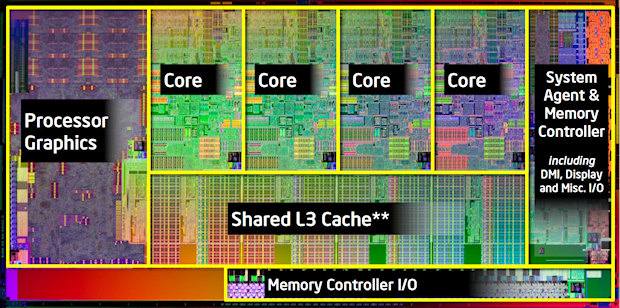
\includegraphics[scale=0.5]{sandy}
  \end{center}
  \caption{
    The figure depicts a quad-core Sandy Bridge microprocessor (or chip). The
    author was unable to locate an image of an octa-core chip.
  }
  \label{fig:p5}
\end{figure}

\subsection{Interconnecting chips to form larger SMPs}

Multiple Sandy Bridge chips can be connected to form larger modules in SMP
configurations. On Vilje, two chips are run in SMP mode on each compute node.
Thus, up to 16 (32) processors share memory.

\subsection{Interconnecting nodes to form a distributed SMP}

Multiple nodes may also be connected to form clusters or distributed SMPs. In
this case, data from one node to another must be passed across a high bandwidth
low-latency switch network. A system based on multiple nodes must therefore be
treated as a distributed memory system (at least globally).

\subsection{Key data for Vilje}

Vilje is based on 1404 nodes. The total number of processors (or cores) is
therefore 22464.

Each node represents a shared memory system with 2 octa-core Sandy Bridge chips
which share 32 GB memory (although a few nodes have 128 GB memory).

Each i7 processor operates at a clock rate of 2.6 GHz. The size of the L1 cache
(3 clocks) is 32 kbyte for data and 32 kbyte for instructions. The size of the
L2 cache (8 clocks) is 256 kbyte, while the size of the shared off-chip L3 cache
is 20 Mbyte.

\section{Programming models}

We have seen that a node (with 16 physical processors) on Vilje represents a
shared memory system where the aggregate memory for the node is globally
available to all the 16 processors. A shared memory programming model (i.e.
OpenMP) can therefore be used within a single node.

If we want to develop programs which can run on more than one node, we need to
use message-passing (i.e. MPI). This is also the programming model we will
emphasize in this course. Even though each node represents a shared memory
system, the message-passing programming model may still be used within a node.
However, the opposite is not true: a shared programming model cannot be used on
a ``pure'' distributed memory system (e.g. on a PC cluster).

Note that a system like Vilje, which represents a shared memory system within a
node, and a distributed memory system across the nodes, can also be programmed
using both programming models within a single program.

\section{Message passing}

Message passing is fundamentally processor-to-processor communication. Only a
local, unique memory is directly available to each processor. Both local and
remote processes must cooperate in order to exchange data and/or synchronize (at
least originally---some changes have been made in the extended version MPI-2).

Note that message-passing is a good way to use distributed shared memory
machines (ccNUMA) because it provides a way to express memory/data locality.

Some of the key advantages of the message-passing model are:
\begin{itemize}
\item {\em Portability}: the model can be used on a collection of
homogeneous or heterogeneous processors connected by a fast or a slow
communication network;
\item {\em Performance}: the approach exploits data locality, as well as the
availability of a large, aggregate memory;
\item {\em Expressiveness}: a limited communcation library suffices for most applications.
\end{itemize}

The Message Passing Interface (MPI) is the de facto standard for message
passing. It is a \emph{library}, not a language. MPI provides efficiency,
portability and functionality. It represents a standardized communcation library
running on a vast number of machines and architectures.
\autoref{fig:message_passing_model} illustrates the message passing model.

The original (1994) MPI-library represents the message passing model where both
the local and remote processes cooperate e.g. via a send and receive
operation. MPI-2 represents an extension of MPI where features like one-sided
messages, parallel I/O, etc. are included.

\begin{figure}
  \centering
  \begin{tikzpicture}[
    proc/.style={shape=circle, draw=darkblue, fill=cadet, thick},
    msg/.style={shape=rectangle, draw=darkblue, fill=cadet, thick, rounded corners=0.5mm},
    env/.style={minimum height=1.7cm, minimum width=1.7cm},
    scale=0.7,
    ]
    \node[proc] (p0) at (0,0) {$P_0$};
    \node[proc] (p1) at (1,3) {$P_1$};
    \node[proc] (p2) at (3,-0.6) {$P_2$};
    \node[proc] (p3) at (6,3.6) {$P_3$};
    \node[msg] (msg) at (4.0, 1.5) {\scriptsize Message};
    \node[msg, env, fill=cadet!55] (env) at (8, -2.0) {};
    \node[msg, very thin] (body) at (8, -1.7) {\scriptsize Body};
    \node[below of=body, node distance=6mm] {\scriptsize Envelope};
    \draw[->, thick] (p2) edge[bend right] node [right] {} (msg);
    \draw[->, thick] (msg) edge[bend right] node [right] {} (p1);
    \draw[->, thick] (env) edge[bend right] node [right] {} (msg);

    \node[msg] (smp) at (-2,-2) {\scriptsize SMP};
    \draw[->, thick] (smp) edge[bend left] node [right] {} (p0);
  \end{tikzpicture}
  \caption{
    The message passing model. A number of processes, $P_0, P_1, \ldots,
    P_{n-1}$, are coupled together via a fast or a slow communication network.
    Each process has a local and unique memory/cache, and each process is
    associated with a particular computational task. The individual processes
    must communicate via explicit message passing. A message consists of an
    ``envelope'' which contains sufficient information about whether and when to
    open the message, as well as information regarding how to interpret the
    ``body'' of the message (the actual data). Note that the message is the only
    means of exchanging data between the processes and/or syncronizing the
    processes.
  }
  \label{fig:message_passing_model}
\end{figure}

The MPI operations can be classified in a few types of operations:
\begin{itemize}
\item one-to-one;
\item one-to-all;
\item all-to-one;
\item all-to-all.
\end{itemize}
The first type is also referred to as point-to-point operations (send and
receive), while the last three types are collective operations.

When we here talk about ``all'', we generally mean all processes $P_0, P_1,
\ldots, P_{n-1}$ within a group of $n$ processes. Such a group defines a
\emph{communicator} and the particular process number is referred to as the
\emph{rank} within that communicator. The default is to let all processes be
members of the same (default) communicator. However, it is also possible to have
some of the processes be members of one communicator (or group), while others be
members of a different communicator. In this context, ``all'' means all the
processes \emph{within} a particular communicator.

Finally, the collective operations can be further broken down into the
following categories:
\begin{itemize}
\item data movement (broadcast; gather/scatter);
\item collective computation (max/min; sum; etc.).
\end{itemize}

We will later explain in more detail the various MPI operations. A good way to
learn MPI is by implementing a few simple examples. The whole library contains
about 125 functions. However, as few as 6 may suffice for some problems. You
only need to learn the functions needed for your particular problem. You may not
have to learn the details of the whole library even for advanced applications.

\subsection{An example}

We now discuss a brief example of a program where the MPI library is used. The
program listed below does the following: processor 0 sends a text message
``Hello, world'' to all the other processors. The other processors receive the
message and all processors print out the message together with the their own
process number.

Listings \ref{lst:mpi-hello-c} and \ref{lst:mpi-hello-fortran} show how this is
done in both C and Fortran.

\begin{lstlisting}[style=c, float, caption={Hello world MPI in C.}, label=lst:mpi-hello-c]
  #include <stdio.h>
  #include "mpi.h"

  int main(int argc, char **argv)
  {
    int rank, size, tag, i;
    MPI_Status status;
    char message[20];

    MPI_Init(&argc, &argv);
    MPI_Comm_size(MPI_COMM_WORLD, &size);
    MPI_Comm_rank(MPI_COMM_WORLD, &rank);

    tag = 100;

    if (rank == 0) {
      strcpy(message, "Hello, world");
      for (i = 1; i < size; i++) {
        MPI_Send(message, 13, MPI_CHAR, i,
                 tag, MPI_COMM_WORLD);
      }
    }
    else {
      MPI_Recv(message, 13, MPI_CHAR, 0,
               tag, MPI_COMM_WORLD, &status);
    }

    printf("node %d: %13s\n", rank, message);

    MPI_Finalize();

    return 0;
  }
\end{lstlisting}

\begin{lstlisting}[style=fortran, float, caption={Hello world MPI in Fortran.}, label=lst:mpi-hello-fortran]
  program hello
  include 'mpif.h'

  integer rank, size, ierror, tag, status(MPI_STATUS_SIZE)
  character(12) message

  call MPI_INIT(ierror);
  call MPI_COMM_SIZE(MPI_COMM_WORLD, size, ierror);
  call MPI_COMM_RANK(MPI_COMM_WORLD, rank, ierror);

  tag = 100;

  if (rank .eq. 0) then
    message = 'Hello, world'
    do i=1,size-1
      call MPI_SEND(message, 12, MPI_CHARACTER, i, tag,
                    MPI_COMM_WORLD, ierror)
    enddo
  else
    call MPI_RECV(message, 12 MPI_CHARACTER, 0, tag
                  MPI_COMM_WORLD, status, ierror)
  endif

  print*, 'node', rank, ':', message

  call MPI_Finalize(ierror)
  end
\end{lstlisting}

The output of the C version on the SGI Origin using $P=4$ and $P=8$ processors
is shown in Listings \ref{lst:mpi-hello-4} and \ref{lst:mpi-hello-8}.

\begin{lstlisting}[float, caption={Hello world MPI in C: $4$ processors.}, label=lst:mpi-hello-4]
  node 1: Hello, world
  node 3: Hello, world
  node 2: Hello, world
\end{lstlisting}

\begin{lstlisting}[float, caption={Hello world MPI in C: $8$ processors.}, label=lst:mpi-hello-8]
  node 5: Hello, world
  node 1: Hello, world
  node 7: Hello, world
  node 2: Hello, world
  node 3: Hello, world
  node 6: Hello, world
  node 4: Hello, world
\end{lstlisting}

Let us now comment on some of the statements here. We start with
\begin{lstlisting}[style=c]
  #include <stdio.h>
  #include "mpi.h"
\end{lstlisting}
The first statement is just a standard statement about including the header file
associated with string (character) operations and I/O. The second statement is
required if we want to use the MPI library in our program. In C, we need the
statement
\begin{lstlisting}[style=c]
  #include "mpi.h"
\end{lstlisting}
The equivalent statement in Fortran is
\begin{lstlisting}[style=fortran]
  include 'mpi.f'
\end{lstlisting}
The MPI header file provides basic MPI definitions and MPI data types.

The first MPI statement needs to be:
\begin{lstlisting}[style=c]
  MPI_Init(&argc, &argv);
\end{lstlisting}
This statement should only be called once. The last MPI statement is always
\begin{lstlisting}[style=c]
  MPI_Finalize();
\end{lstlisting}
This statement does not have to be the very last statement in your program, but
it needs to be the last MPI statement. It statement ensures a clean exit.

Note that the command line arguments are passed to the C version of
\texttt{MPI\_Init}. The corresponding Fortran version reads:
\begin{lstlisting}[style=fortran]
  call MPI_INIT(ierror);
\end{lstlisting}
Similar to a standard subroutine call in Fortran, a call to an MPI operation
also starts with \texttt{call}. The parameter \texttt{ierror} is an integer and
will return an error code in case something goes wrong. The C version also
returns an error code. Instead of the statement used in the program listed
above, we could alternatively have written
\begin{lstlisting}[style=c]
  errorcode = MPI_Init(&argc, &argv);
\end{lstlisting}
In this case, the variable \texttt{errorcode} (an integer) will contain an error
code if something goes wrong.

In general, any MPI statement in C has the format
\begin{lstlisting}[style=c]
  errorcode = MPI_Xxxxx(parameters...);
\end{lstlisting}
or simply
\begin{lstlisting}[style=c]
  MPI_Xxxxx(parameters...);
\end{lstlisting}
The particular MPI operation is given by ``Xxxxx'' where the name of the operation
always starts with a capital letter and the remaining letters are lower-case.
The number and type of parameters vary from operation to operation. For example,
\texttt{MPI\_Finalize} does not have any parameters at all.

In Fortran, any MPI statement has the format.
\begin{lstlisting}[style=c]
  call MPI_XXXXX(parameters..., ierror)
\end{lstlisting}
where the parameter \emph{ierror} returns an error code. Note that the name of
the particular MPI operation is always in capital letters.

The next two statements after the initialization of MPI are:
\begin{lstlisting}[style=c]
  MPI_Comm_size (MPI_COMM_WORLD, &size);
  MPI_Comm_rank (MPI_COMM_WORLD, &rank);
\end{lstlisting}
The first of these statements returns the total number of MPI processes, while
the second one returns the individual process number (the ``rank''). More
precisely, the process number is stored in the location pointed to by the second
argument. \texttt{MPI\_COMM\_WORLD} is the default name of the communicator (the
``univertse'') and which include all the processes. This can be changed in order
to create several separate ``universes.''

Note that the program listed in this example runs separately and independently
on every processor on a multiprocessor. We also refer to this as SPMD -
\emph{Single Program Multiple Data}. All the problems we will study in this
course will be of this type: the program running on each processor will be the
same for all the processors. However, the data each processor will operate on
will typically be different. The synchronization of the program will be implicit
via the MPI operations. We will return to this issue later.

When this program runs on a particular processor, the program does not
automatically know how many other processors are involved; this issue is taken
care of by the MPI operation \texttt{MPI\_Comm\_size}. In the multiprocess
context, the program running on an individual processor does not automatically
know what its associated process number is (who am I?); this issue is taken care
of by the MPI operation \texttt{MPI\_Comm\_rank}.

Let us now proceed to the statements
\begin{lstlisting}[style=c]
  if (rank == 0) {
    strcpy (message, "Hello, world");
\end{lstlisting}
The if-statement will only be true for one of the processes, namely, the process
with process number 0. This is also referred to as the ``root'' process. On the
root process, the string ``Hello, world'' is copied into the string variable
\texttt{message}.

For all the other processes, the if-statement will not be true, and the program
execution will move on to the MPI statement \texttt{MPI\_Recv}. This means that
all of the other processes will be waiting for the root process to send them
data. The root process sends data to the other processes in the loop
\begin{lstlisting}[style=c]
  for (i=1; i < size; i++) {
    MPI_Send(message, 13, MPI_CHAR, i,
             tag, MPI_COMM_WORLD);
  }
\end{lstlisting}
Several comments are in order here. First, note that the root process sends out
the same message (string) to all the other processes. This is done in a loop.
However, note that this loop corresponds to a \emph{sequential} execution
meaning that a message will be sent to process $1$ before process $2$ etc.

Let us now discuss the particular format in the parameter list for the operation
\texttt{MPI\_Send}. The general format for this operation is
\begin{lstlisting}[style=c]
  MPI_Send(start, count, datatype, dest, tag, comm);
\end{lstlisting}
The first three parameters (start, count, datatype) represent \emph{the data},
while the last three parameters (dest, tag, comm) represent \emph{the envelope};
see \autoref{fig:message_passing_model}.

We now explain all these parameters in some more detail.
\begin{itemize}
\item \emph{start}: initial address of the send buffer
\item \emph{count}: number of elements sent (of type \texttt{datatype})
\item \emph{datatype}: e.g. \texttt{MPI\_INT}, \texttt{MPI\_FLOAT}, \texttt{MPI\_CHAR} etc.
\item \emph{dest}: destination process (integer)
\item \emph{tag}: integer message identifier (e.g., \texttt{MPI\_ANY\_TAG})
\item \emph{comm}: an ordered group of communication processes (same for send
  and receive)
\end{itemize}

Only the root process sends a message. All the other processes are waiting to
receive a message. This is expressed by the MPI operation \texttt{MPI\_Recv}.
The general format for this operation is
\begin{lstlisting}[style=c]
  MPI_Recv(start, count, datatype, source, tag, comm, &status);
\end{lstlisting}
The first three parameters (start, count, datatype) represent \emph{the data},
while the last three parameters (dest, tag, comm, status) represent \emph{the
envelope}; again, see \autoref{fig:message_passing_model}.

Most of the parameters are similar to the MPI\_Send operation:
\begin{itemize}
\item \emph{start}: initial address of the receive buffer
\item \emph{count}: number of elements sent (of type \emph{datatype})
\item \emph{datatype}: e.g. \texttt{MPI\_INT}, \texttt{MPI\_FLOAT}, \texttt{MPI\_CHAR} etc.
\item \emph{source}: source process (integer), i.e., the process sending the message
\item \emph{tag}: integer message identifier (e.g., \texttt{MPI\_ANY\_TAG})
\item \emph{comm}: an ordered group of communication processes (same for send and receive)
\item \emph{status}: a structure providing information on the completed communication
\end{itemize}

Note that in the small example program, an explicit source is given, namely, the
root process. Alternatively, we could have used \texttt{MPI\_ANY\_SOURCE} since
each process in receive mode only expects one message. Similarly, we note that
the ``tag'' is explicitly given. Alternatively, we could have used
\texttt{MPI\_ANY\_TAG} since this parameter is not critical in our case.

One additional comment regarding the send and receive statements. This is an
example of point-to-point communication. There exists several versions of send
and receive. The type used here is called \emph{blocking} send and receive. This
means that the program running on the root processor cannot proceed until each
message has been safely sent and the send buffer can be safely used again.
Similarly, the program running on each of the other processors cannot proceed
until the expected message has been received in the receive buffer.

Let us now comment on the parameter \emph{count} used in the send and receive
statements. In the C version, the count parameter is set equal to 13, while it
is 12 in the Fortran version. The reason for this is that the \texttt{strcpy}
function in C will append \texttt{\textbackslash 0} (the null character) at the
end of the message. This is a symbol which indicates the end of the string. Even
though ``Hello, world'' comprises 12 letters (one byte per letter), the message
buffer in C requires 13 bytes of memory.

The parameter ``datatype'' in the send and receive operations has to be the same.
In this case, the type is \texttt{MPI\_CHAR} (in Fortran the corresponding data
type is called \texttt{MPI\_CHARACTER}). This is one of several predefined data
types. Other important ones include \texttt{MPI\_DOUBLE} and \texttt{MPI\_INT}.

Finally, note that the output from the programs is not in a sequential order.
The order may also change if we run the program over again.


% \begin{thebibliography}{99}

% \bibitem {} D.E. Culler and J.P. Singh, Parallel Computer Architecture,
% {\em Morgan Kaufmann Publishers, Inc.}, 1999.

% \bibitem {} C.C. Douglas, G. Haase, J. Hu, M. Kowarschik, U. Rude,
% and C. Weiss, Portable memory hierarchy techniques for PDE solvers: Part I,
% {\em SIAM News}, Vol. 33, No. 5, 2000.

% \bibitem {} B. Lande, Optimalisering av flyttallsintensive programmer,
% Institutt for matematiske fag, NTNU, 2004. (In Norwegian.)

\end{document}
